\chapter{Méthodologie}
\minitoc%

\section{Données Fonctionnelles : l'essentiel}
\label{sec:fda_essentiel}

\subsection{Définitions et propritétés informelles}
\label{sec:informel}
% ⚠️ obsolète dû au remaniement des parties et annexes
% Commençons par introduire les données fonctionnelles de manière informelle afin de mieux intégrer la définition formelle, plus utile pour la manipulation.

Nous allons dans cette section introduire la notion de donnée fonctionnelle ainsi que les propriétés les plus utiles lorsqu'on les manipule. On y regroupe l'ensemble des messages essentiels à retenir des données fonctionnelles pour la pratique, sans alourdir les notions avec des notations mathématiques. Le cadre formel est traîté en annexe ~\ref{annexe:fda-formel}.

\begin{definition*}[données fonctionnelles — informel]
	Les données fonctionnelles sont des données dont les observations sont des fonctions, c'est-à-dire des courbes, des surfaces, des images, \, \dots

	i.e : toute donnée ayant une dépendance de type "relation fonctionnelle" avec un ou plusieurs paramètres.
	\label{def*:fda}
\end{definition*}

\begin{figure}[H]
	\begin{center}
		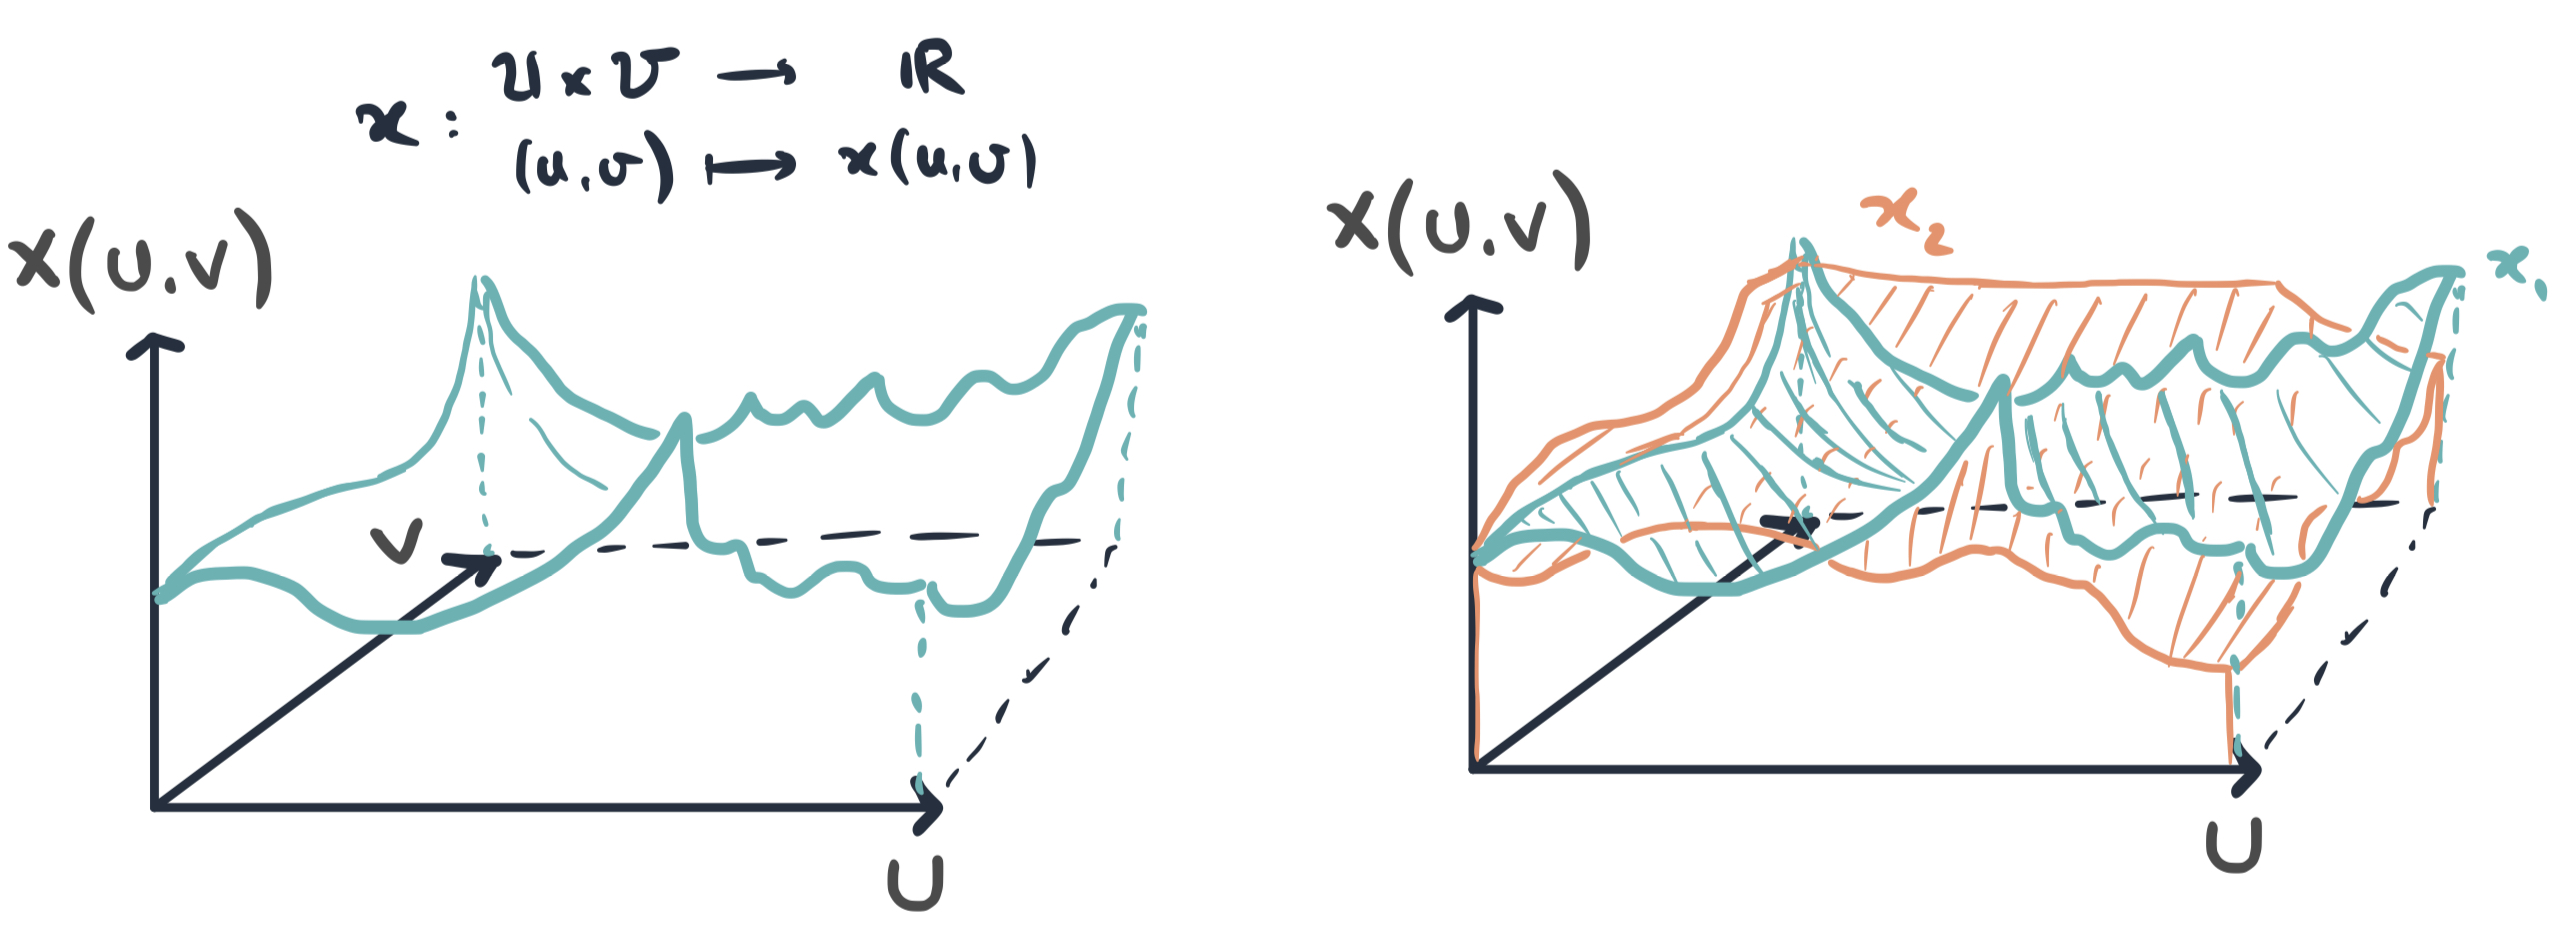
\includegraphics[width=0.8\textwidth]{Images/sketches/fda_surface.jpg}
	\end{center}

	{
	\textbf{Gauche :} exemple de surface
	\\
	\textbf{Droite :} échantillon de deux observations de la surface suivant une loi fonctionnelle}

	\caption{Donnée fonctionnelle : relation fonctionnelle avec plusieurs paramètres}
	\label{fig:sketch_surface}
\end{figure}

Maintenant introduites, les théorèmes suivant permettent de manipuler ces données à la fois pour la théorie et la pratique :

\begin{thm*}[\nameref{thm:KL} — informel]
	\noindent\fbox{%
		\parbox{\textwidth}{%
			Il est possible pour une large classe de données fonctionnelles de les décomposer dans une base \emph{de fonctions} adaptée aux données (au sens de la covariance) que l'on appelle base ACP fonctionelle (FPCA).
		}%
	}
	\label{thm*:KL}
\end{thm*}


\begin{rem}
	La classe de fonctions pouvant être décomposées est large, puisqu'elle regroupe l'ensemble des processus qui nous intéressent la plus part du temps en tant que statisticien : celles qui sont à support sur un intervalle, admettant une covariance continue et finie sur le support.
\end{rem}

On en déduit que pour travailler avec des données fonctionnelles, il suffit de les décomposer dans la base ACP fonctionnelle puis de travailler sur les composantes de chaque élément de la base. On travaille désormais avec des réels et non plus des fonctions, ce qu'on aime manipuler. On peut alors faire de la statistique traditionnelle avec les outils que l'on connait.


\begin{propriete*}[intérêt de la base FPCA — informel]
	\noindent\fbox{%
		\parbox{\textwidth}{%
			la base ACP fonctionnelle est la plus économe, c'est à dire qu'elle explique au mieux la covariance des données pour un nombre de composantes fixées, ce qui est utile car on ne sait manipuler numériquement que des objets de dimension finie.
		}%
	}
\end{propriete*}

Pour avoir une bonne représentation de ces données, on doit donc s'assurer de bien estimer la covariance. Pour cela, on a mentionné qu'il serait judicieux de lisser les observations en tenant compte de la régularité du processus dont est issu nos données. La question est désormais la suivante :

\question{
	Est-il possible de récupérer la régularité locale des trajectoires à partir des données ? Si oui, comment ?
}

C'est ce qu'affirme le théorème suivant provenant des travaux de Golovkine et MPV :

\bigskip

% TODO : créer un alias samepage 
% \samepage{stuff} = \noindent\begin{minipage}{\textwidth} stuff \end{minipage}
\noindent\begin{minipage}{\textwidth}
\begin{thm*}[Regularité locale — informel]
	\noindent\fbox{%
		\parbox{\textwidth}{%
			Les données fonctionnelles permettent de récupérer la régularité locale des trajectoires. Les estimateurs définis \textbf{ponctuellement} convergent.
		}%
	}
	\label{thm*:regularite_locale}
\end{thm*}
\end{minipage}
\begin{rem}[Continuité de Kolmogorov]
	Un théorème (\nameref{thm:kolmogorov_continuite}) permet à partir de l'espérance d'incréments d'un processus aléatoire de déduire sa régularité.
	C'est pourquoi les estimateurs sont définis à partir des incréments quadratiques. C'est entre autres \emph{la raison pour laquelle les données fonctionnelles permettent de récupérer la régularité locale des trajectoires}.

	\label{rem:kolmo_continuite}
\end{rem}


% \subsection{estimation adaptative informelle}
% Les motivations de l'obtention de la régularité étaient en partie de pouvoir mieux estimer les quantités qui nous intéressent dont la fonction moyenne du processus, ainsi que son opérateur de covariance. Ce qui est à la fois important pour l'analyse (via l'interprétation de la base ACP déterminée par la covariance) et pour la prédiction. On peut alors se demander si il existe des estimateurs de la moyenne et de la covariance prenant en compte la régularité locale. C'est ce qu'affirme les théorèmes suivants :

\warn{demander à Hassan la dernière version de son papier car la partie d estimation adaptative a beaucoup changé}

\begin{thm*}[Estimateurs de la moyenne et de la covariance — informel ~\cite{golovkine2021adaptive}]
	\noindent\fbox{%
		\parbox{\textwidth}{%
			Il est possible en lissant les observations par méthode à noyaux avec une largeur de bande \emph{spécifique à l'objet que l'on souhaite estimer}, de dériver des estimateurs de la moyenne et de la covariance qui convergent.
			La largeur de bande optimale \emph{pour l'objet que l'on souhaite estimer} est celle qui minimise un risque qui effectue un compromis biais-variance, qui dépend de la régularité locale du processus, en pénalisant les largeurs de bande menant à des "trous" dans les fonctions lissées.
			On parle d'\emph{\og estimation adaptative \fg}.
		}%
	}

	\label{thm*:estimation_adaptative}
\end{thm*}

Cependant, bien qu'une largeur de bande optimale existe, elle est inconnue. Il est donc important de savoir si le praticien peut l'estimer, et avec quelle précision (c'est à dire à quel point l'estimateur sera biaisé ou non). C'est ce que nous affirme le théorème suivant :

\begin{thm*}[expression de la largeur de bande optimale — informel ~\cite{golovkine2021adaptive}]
	\noindent\fbox{%
		\parbox{\textwidth}{%
			Sous certaines hypothèses de régularité du processus, et d'indépendance des temps observés, la largeur de bande optimale peut être approchée (avec forte probabilité de bonne approximation) par une expression ne dépendant que du nombre de courbes observées, du nombre moyen de temps observés par courbe, et de la régularité locale du processus. Ce biais de l'estimateur de la fonction moyenne est alors contrôlé en fonction de ces mêmes quantités.

			Sous des hypothèses un peu plus fortes sur la relation entre le nombre moyen d'observations par courbe et le nombre de courbes, on dispose de résultats similaires pour l'estimateur de la covariance.}%
	}

	\label{thm*:h_opt_estim}
\end{thm*}


Enfin, on peut se demander ce qu'il en est des estimateurs dans le cadre où l'on dispose de la dépendance dans les données (ce qui est la cas pour les données éoliennes notamment). Ce cas est traîté par le théorème suivant dérivé par MPV :

\begin{thm*}[ Estimation adaptative de séries temporelles fonctionnelles — informel ~\cite{maissoro-SmoothnessFTSweakDep} ]

	On peut estimer la régularité d'une série temporelle de données fonctionnelles à condition que la mémoire temporelle de la série soit courte. (La décroissance de la dépendance temporelle doit être au moins aussi rapide qu'une décroissance géométrique)

	\label{thm*:far_adaptative_estimation}
\end{thm*}

% \pagebreak

\subsection{Résumé de l'intérêt de la modélisation fonctionnelle}

Les données fonctionnelles permettent de travailler sur un modèle où la \emph{relation} entre plusieurs quantités est sujet à une loi \footnote{$cf$ \nameref{def*:fda} : \ref{def*:fda}}. Ce point de vue de réplication de courbes est notamment utile car il permet d'extraire des observations leur régularité\footnote{$cf$ \nameref{rem:kolmo_continuite}, \nameref{thm*:regularite_locale} : \ref{rem:kolmo_continuite}}. L'estimation de cette régularité permet, entre autres, de lisser les courbes de façon appropriée en fonction de la quantité que l'on souhaite estimer, telle que la moyenne et la covariance avec une plus grande précision\footnote{$cf$ \nameref{thm*:estimation_adaptative} : \ref{thm*:estimation_adaptative}}.

\noindent\begin{figure}[H]
	\centering
	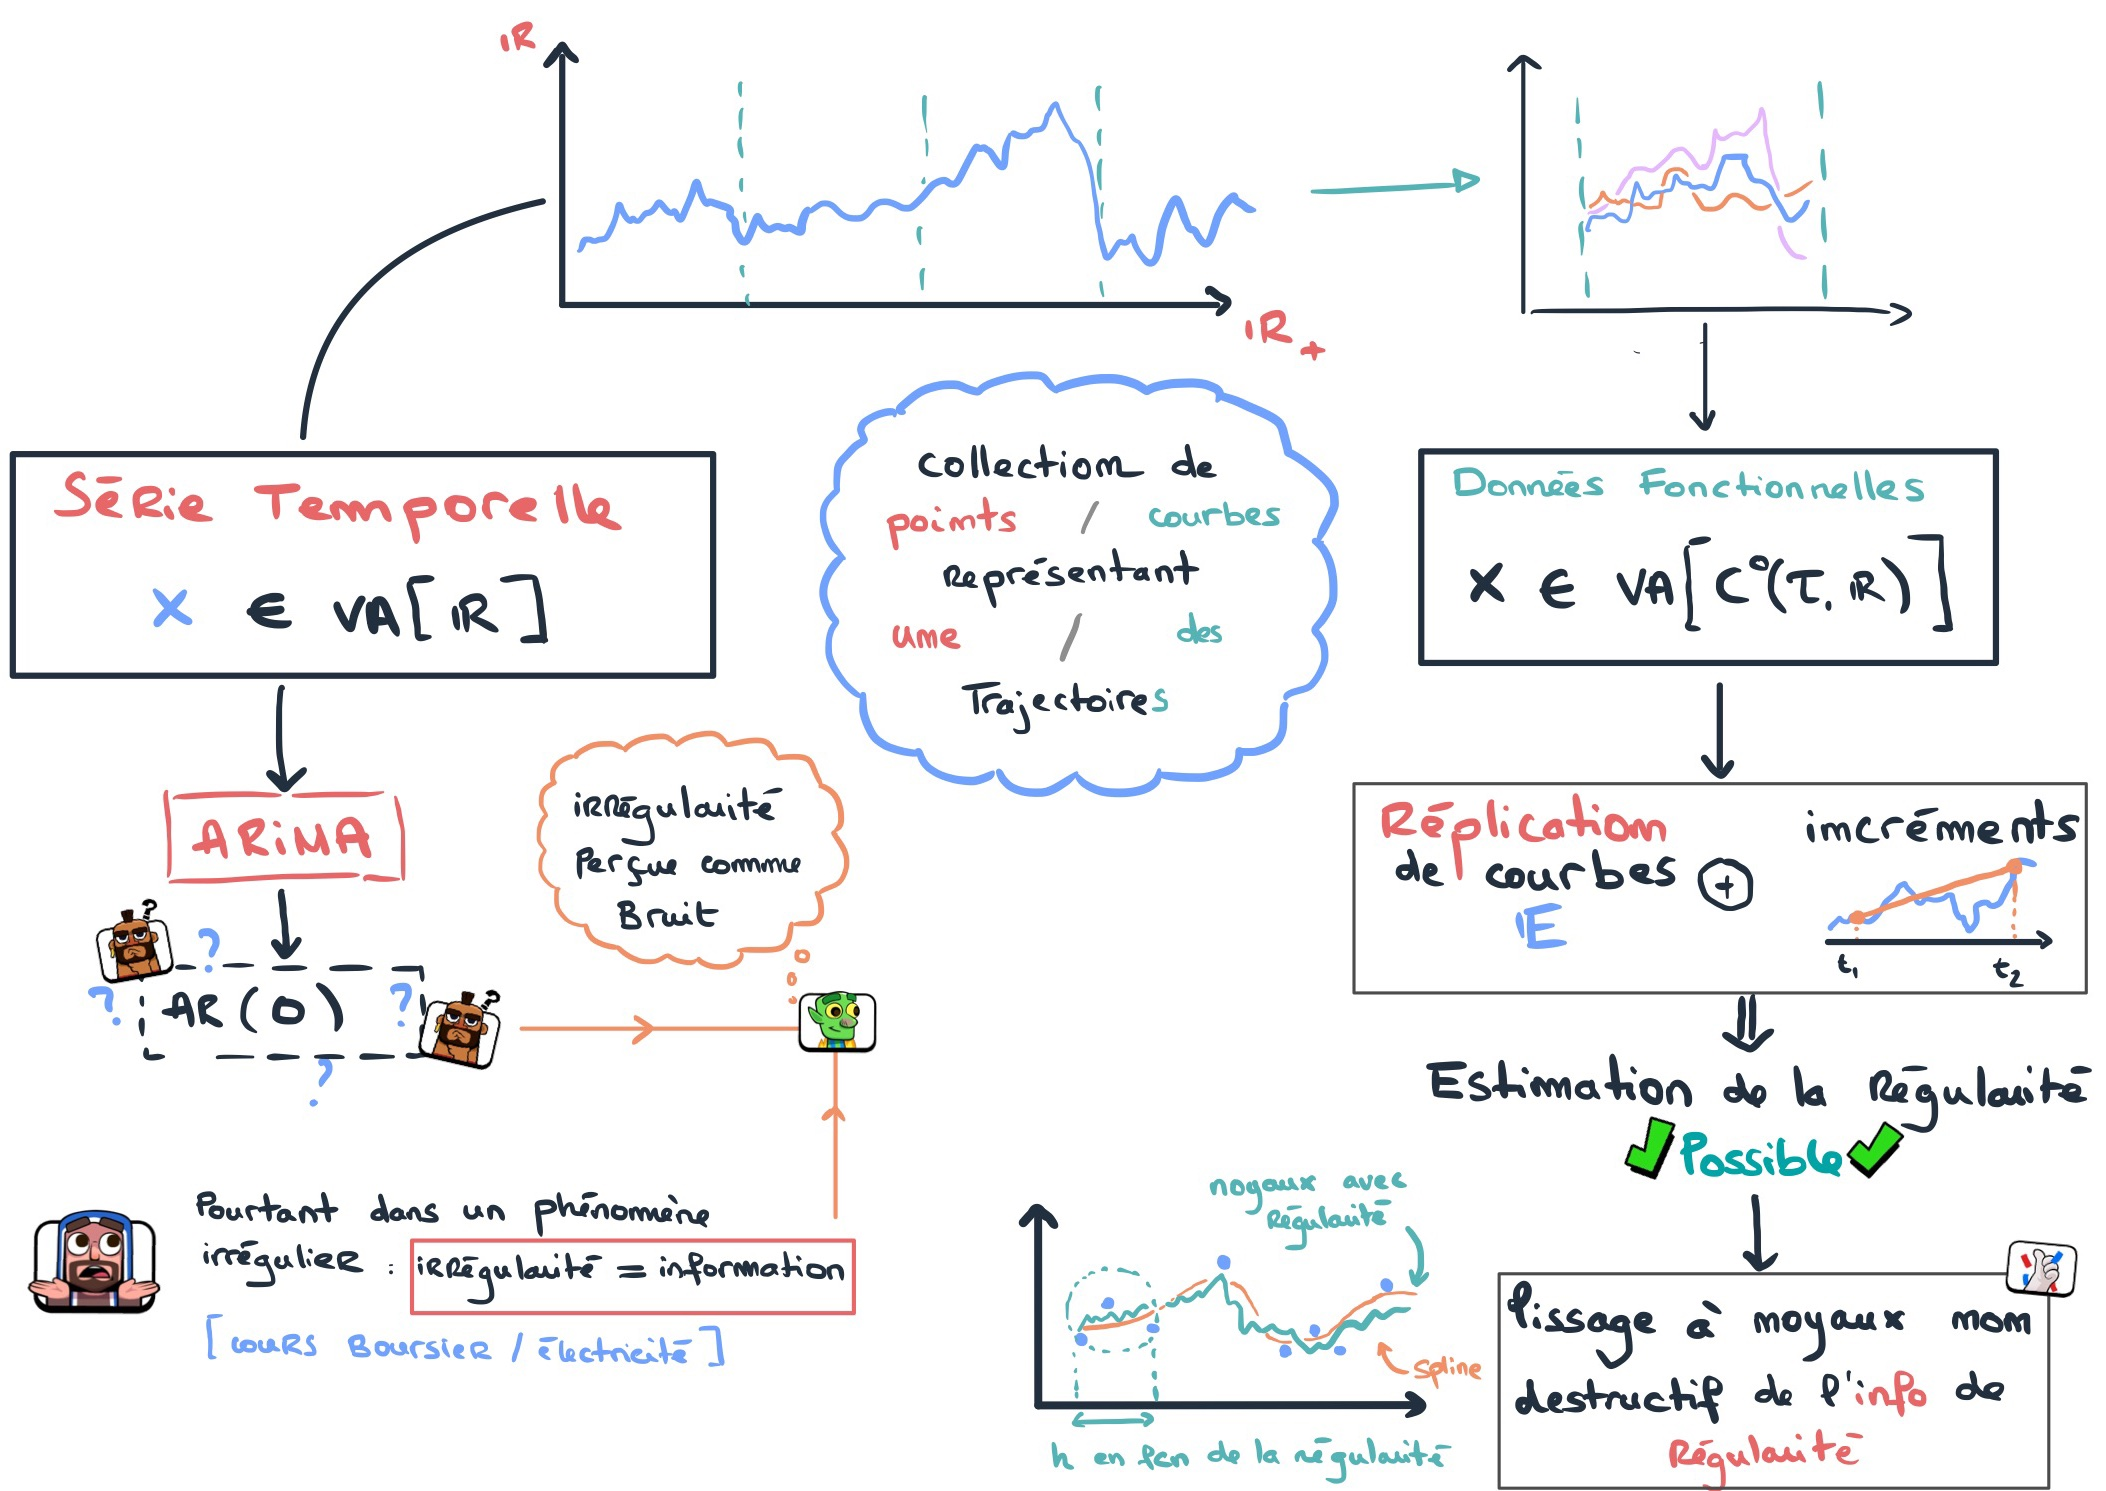
\includegraphics[width=0.8\textwidth]{Images/sketches/sketch_resume_informel.jpeg}
	\caption{Résumé des motivations du de l'estimation de la régularité locale des trajectoires}
	\label{fig:sketch_resume_informel}
\end{figure}

\pagebreak

% \subsection{Données fonctionnelles : formellement}
% \subsubsection{Définition formelle}

Pour éviter d'alourdir les notations, on se place dans le cas où les fonctions sont à valeurs dans $\mathds R$ et à support sur un intervalle fermé $I$ de $\mathds R$. Toutefois, on peut très bien considérer des fonctions à valeurs dans $\mathds R^d$ et à support sur un compact $K$ de $\mathds R^p$ sans perte de généralités.

\begin{definition}[données fonctionnelles ]

    On appelle données fonctionnelles, un échantillon $\famfinie x 1 n$ de fonctions continues $x_i : I \rightarrow \R d$ issues d'un processus $X$ défini comme ci-dessous :

    $$X :
        \begin{array}{ccc}
            \Omega & \longrightarrow & \mathcal C(I, \mathds R)
            \\
            \omega & \longmapsto     & X(\omega) = x
        \end{array}
    $$

\end{definition}

\subsubsection{Résultats importants}

On énonce désormais le théorème central de l'analyse de données fonctionnelles qui n'est autre que la décomposition dans la base FPCA de notre processus.

\begin{rem}
	on notera que dans le cadre des données fonctionnelles, on ne travaille pas de façon générale avec la covariance :

	$$C_X : (s,t) \mapsto \esperance{ \left[X - \mu\right](s) \cdot \left[X - \mu\right](t) }$$

	On travaille plutôt avec l'\textbf{opérateur} de covariance :

	\begin{equation*}
		c : \begin{array}{ccc}
			\mathds L^2 & \longrightarrow & \mathds L^2                             \\
			f           & \longmapsto     & \int\limits_I f(u)C_X(u, \cdot \,) \,du
		\end{array}
	\end{equation*}

	C'est parceque cet opérateur est linéaire continu (car Hilbert-Schmidt donc borné pour la norme d'opérateur) symétrique semi-défini positif (pour le produit scalaire de $\mathds L^2$) et que l'on peut donc en faire une décomposition spectrale sur une base orthonormale de vecteurs propres associés à des valeurs propres positives. Cette décomposition est à la base des approximations que le praticien effectuera ainsi qu'à la base de la dérivation de nombreux théorèmes et propriétés.
\end{rem}

\bigskip

Etant donné que l'on traîte des données fonctionnelles, on considère la géométrie usuelle de $\mathds L^2(\mathds R, \, \lambda)$ et on note ainsi

\begin{equation*}
	\prodscalselon \cdot \cdot {\mathds L^2}: \begin{array}{ccc}
		\mathds L^2 \times \mathds L^2 & \longrightarrow & \mathds R
		\\
		(f,g)                          & \longmapsto     & \int f(u)g(u) \, d\lambda(u)
	\end{array}
\end{equation*}


le produit scalaire que l'on considère pour manipuler les données fonctionnelles.


% https://stackoverflow.com/a/4008463 : no page break
\begin{minipage}{\textwidth}
	\begin{thm}[Karhunen-Loeve]
		\emph{référence :} ~\cite[pages : 238-239-241]{kokoszka2017introduction}

		\textbf{Hypothèses :}

		\begin{equation*}
			\boxed{
				\begin{array}{ll}
					\textsf{\faCaretSquareRight} & X \in \mathds L^2( \Omega, \mathcal C(I, \mathds R))
					\\ \\
					\textsf{\faCaretSquareRight} & \textsf{covariance : } C : \begin{array}{ccc}
						                                                          \mathds L^2( \Omega, \mathcal C(I, \mathds R)) & \longrightarrow & \mathcal C(I^2, \mathds R)
						                                                          \\
						                                                          X                                              & \longmapsto     & C_X
					                                                          \end{array}
					\\ \\
					                             & \textsf{ie : } C_X : (s, t) \mapsto C_X(s,t) \textsf{ est continue}
					\\ \\
					\textbf{\faIcon{asterisk}}   & \textsf{opérateur covariance} \, c_X[ \, \cdot \, ] : \begin{array}{ccc}
						                                                                                     \mathcal C(I, \mathds R) & \longrightarrow & \mathcal C(I, \mathds R)
						                                                                                     \\
						                                                                                     f                        & \longmapsto     & \int_I f(s) C_X(s, \cdot \, ) \, ds\end{array}
					\\\\
					\textsf{\faCaretSquareRight} & \textsf{valeurs propres ordonnées : } \forall p \geq 1, \lambda_{p+1} \leq \lambda_p \quad\quad \lambda_p, \lambda_{p+1} \in \operatorname{sp}(c_X)
					\\ \\
					\textbf{\faIcon{asterisk}}   & \textsf{on pose } \overrightarrow{sp}_{\orthonormal}^{[1,p]}(c_X) \isdef \left\{ \phi_k \in \overrightarrow{sp}_{\orthonormal}( \, c_X \, ) \textsf{ associé à }  \lambda_k, k \in \intervaleint 1 p \, \right\}
				\end{array}
			}
		\end{equation*}

		\textbf{alors :}
		\begin{equation*}
			\boxed{
				\begin{array}{cc}
					\textsf{\faCaretSquareRight} &

					\forall p \geq 1
					\quad
					\argmin\limits_{u_k \in \mathcal C(I, \mathds R)} \mathds E \left\Vert X - \sum\limits_{k=1}^p \prodscalselon {X - \mu} {u_k} {\mathds L^2} u_k \right\Vert^2 = \overrightarrow{sp}_{\orthonormal}^{[1,p]}( \, c_X \, )

					\\
					\\
					\textsf{\faCaretSquareRight} & X = \mu + \sum\limits_{k=1}^{+\infty} \prodscal {X - \mu} {\phi_k} \phi_k
					\\
					                             &
					\\
					                             & \textsf{avec } \phi_k \in \overrightarrow{sp}_{\orthonormal}( \, c_X \, )
				\end{array}
			}
		\end{equation*}

		\label{thm:KL}
	\end{thm}
\end{minipage}
\begin{proof}[\faCogs \, preuve informelle]
	La covariance est un opérateur bilinéaire symétrique défini positif, on peut donc appliquer le théorème de Mercer (équivalent du théorème spectral) qui nous donne une base orthonormale de $\mathds L^2$ sur laquelle on va décomposer notre processus \textbf{centré}.
\end{proof}


\begin{rem}
	pour pouvoir ordonner les valeurs propres dans l'ordre décroissant, et sélectionner les composantes principales les plus informatives, il faut pouvoir réarranger l'ordre de la somme. Pour cela il faut que les valeurs propres forment une famille sommable, une condition suffisante et souvent utilisée est que $\mathds E \Vert X \Vert^2 < \infty$
\end{rem}

\begin{rem}
	la propriété de la section précédente sur l'aspect économe de la base FPCA découle directement de l'assertion
	\begin{equation*}
		\forall p \geq 1
		\quad
		\argmin\limits_{u_k \in \mathcal C(I, \mathds R)} \mathds E \left\Vert X - \sum\limits_{k=1}^p \prodscal {X - \mu} {u_k} u_k \right\Vert^2 = \overrightarrow{sp}_{\orthonormal}^{[1,p]}( \, c_X \, )
	\end{equation*}
	dans le théorème de Karhunen-Loeve.
\end{rem}



% \pagebreak

\subsection{Cas non indépendant : séries temporelles de données fonctionnelles}
Une large partie de la théorie des données fonctionnelles suppose que l'on observe des courbes $X_i : \Omega \rightarrow \mathcal C^0(I, \mathds R)$ \textbf{indépendantes} et identiquement distribuées. Cependant une partie non négligeable des données que l'on observe ont des dépendances avec les valeurs passées. Par exemple, il est raisonnable de penser que la consommation électrique d'un foyer au cours d'une année croît avec l'ajout successif de nouveau appareils électroniques. L'hypothèse d'indépendance entre les données n'est donc plus pertinente pour les données que l'on traite et il devient important de considérer des processus autorégressifs adaptés aux données fonctionnelles.
Si dans le cadre des données de $\mathds R$ cette relation de \emph{dépendance linéaire} avec le passé pouvait s'écrire sous la forme suivante
$X_n = \sum\limits_{k=1}^{n-1} \varphi_k \, X_k + \xi_n$ où $\varphi_k \in \grandR$
et
$\xi_n \begin{cases} \in \operatorname{VA}(\grandR) \\ \indep \sigma\left( X_i \right)_{1\,: \, n-1}\end{cases}$,
dans le cadre fonctionnel on capture la même idée en considérant
$X_n = \sum\limits_{k=1}^{n-1} \phi_k \left( X_k \right) + \xi_n$ où $\phi_k$
est un \emph{opérateur linéaire} de $\mathds L^2(I, \mathds R)$,
le plus souvent intégral.

\chk{
	Il s'agit d'une généralisation naturelle de la relation dans le cadre réel, puisqu'on peut démontrer que sur l'espace des nombres réels l'ensemble des fonctions linéaires $\phi : \grandR \rightarrow \grandR$ sont de la forme $x \mapsto ax$ avec $a \in \grandR$. La relation sur $\grandR$ que l'on a vue juste avant peut alors se ré-écrire de façon similaire à la version fonctionnelle.
}

On considère lors de ce stage des séries temporelles de données fonctionnelles car les données que l'on manipule ( en l'occurence les données de courbe de charge des parcs éoliens ) semblent être naturellement corrélées dans le temps.


\question{Pourquoi se soucier en particulier des séries temporelles fonctionnelles lorsque l'on souhaite incorporer la régularité du processus dont est issu nos données dans l'estimation des quantités qui nous intéressent ?}

Rappelons-nous que les données fonctionnelles sont la clé pour déterminer la régularité, et que cela est en réalité permis par le théorème de \nameref{rem:kolmo_continuite} (que nous n'avons pas énoncé en détails, mais mentionné dans la section \ref{sec:informel}). Malheureusement, dans le monde réel où vit le praticien, nous n'avons pas accès à l'espérance de la loi dont sont issues nos données. Il nous faut donc estimer cette espérance, et c'est là que les séries temporelles fonctionnelles entrent en jeu. Puisque l'estimateur usuel de l'espérance est la moyenne empirique, qui nous est fourni par la loi des grands nombres, cela devient très problématiques lorsque l'on dispose de données corrélées.
% TODO ✏️ mieux formuler - dépendance faible -> LGN faible -> estim esperance
Ce que nous allons voir, c'est que l'on peut tout de même utiliser l'estimateur usuel de l'espérance, et que l'on obtiendra des estimateurs des paramètres de régularité convergents ponctuellement vers ceux du processus dont sont issues nos données. Ce résultat est dérivé en utilisant une forme particulière de dépendance que le lecteur pourra étudier plus en détail en annexe \ref{annexe:regularite-locale}.

\begin{figure}[H]
	\centering
	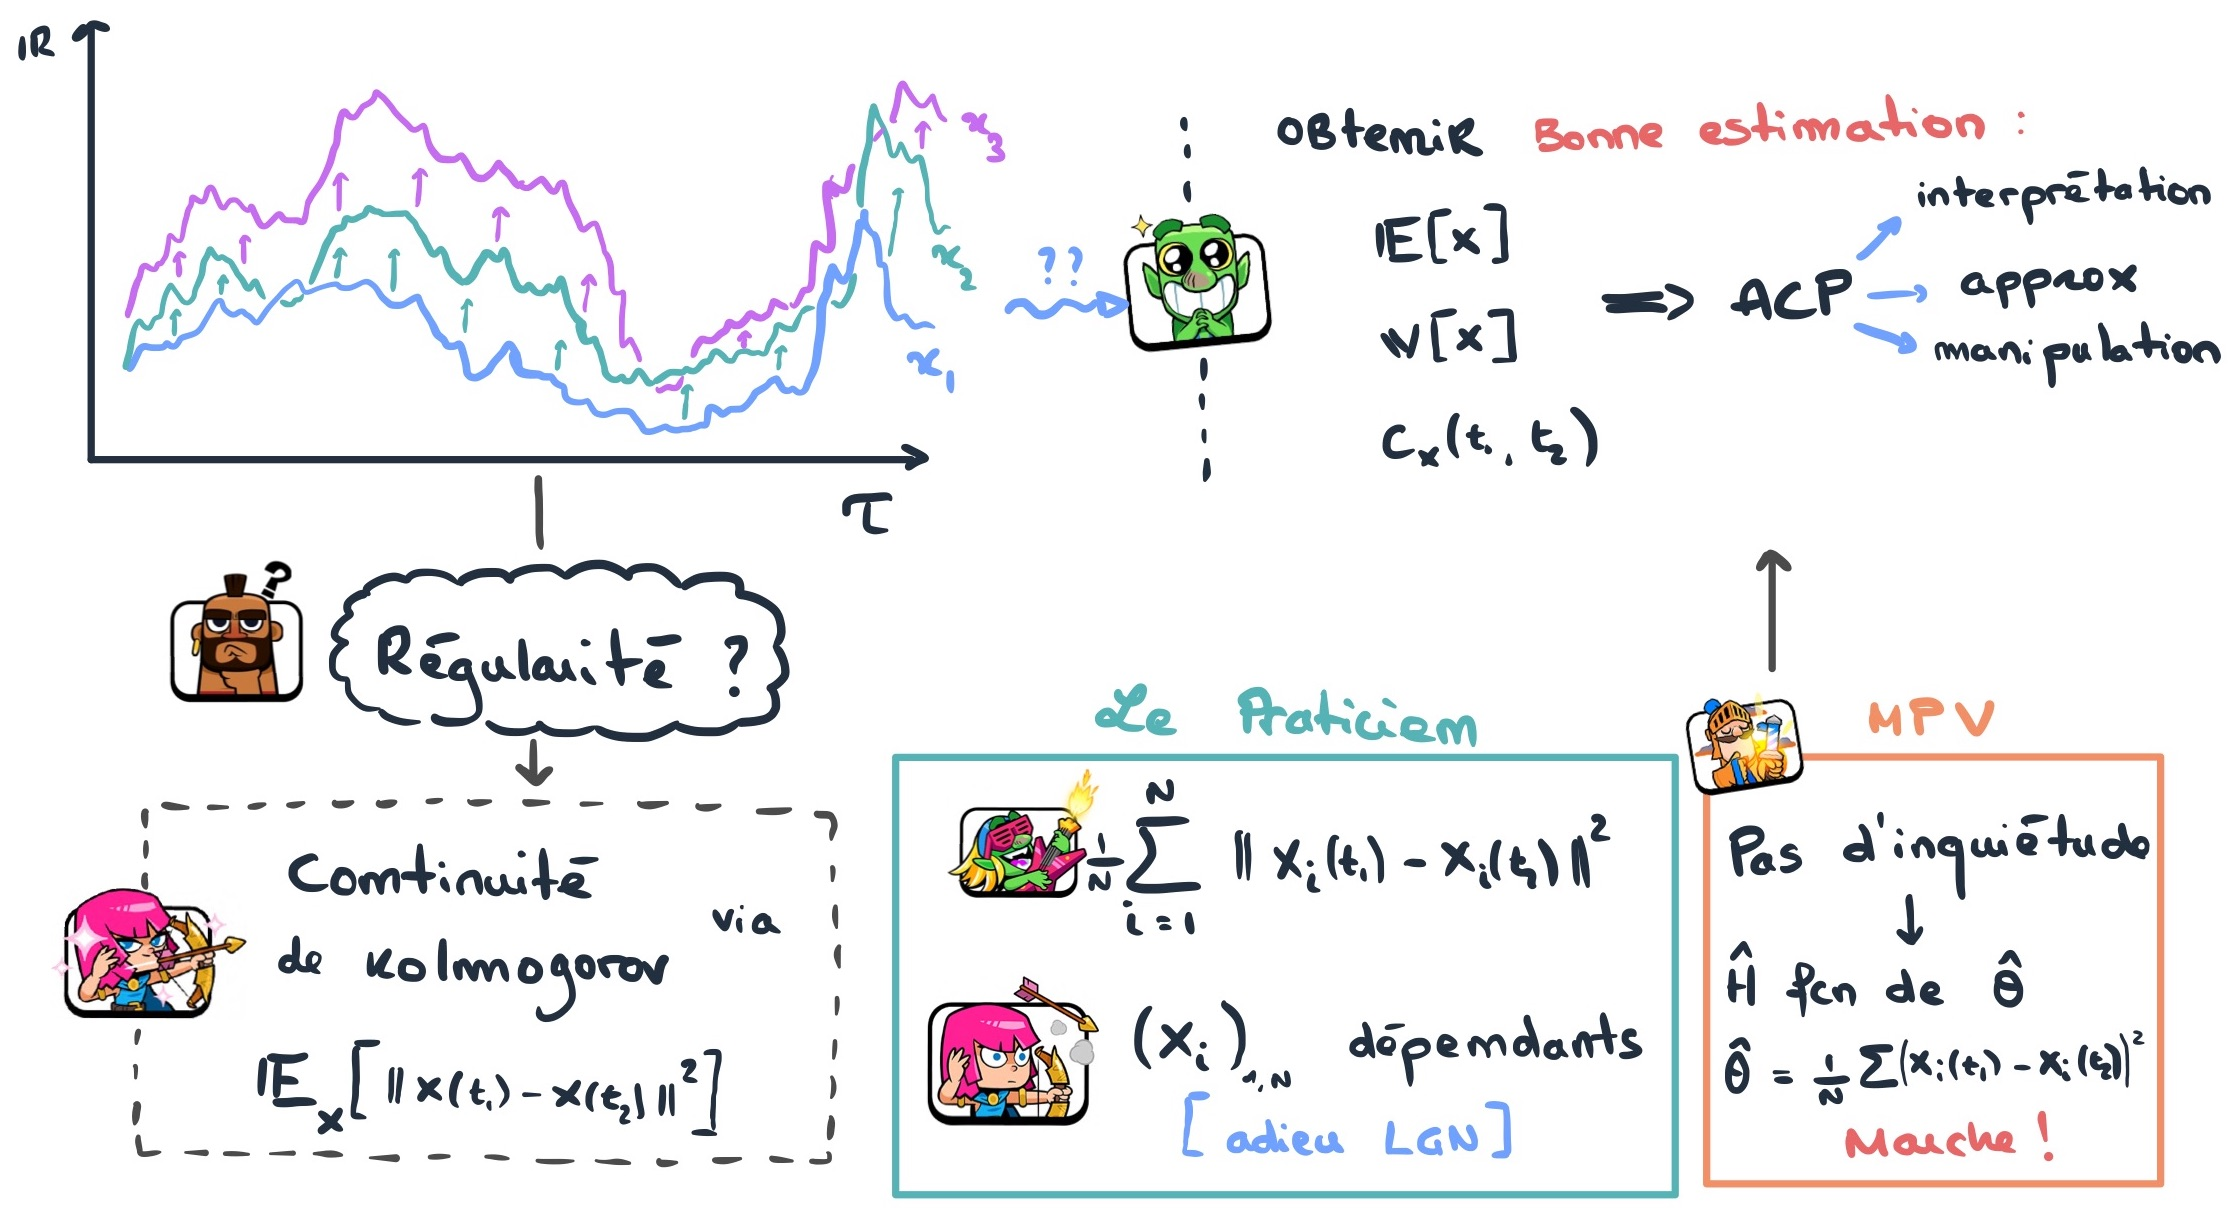
\includegraphics[width=\textwidth]{Images/sketches/schema_ts_estim_reg.jpg}
	\caption{Schéma grossièrement récapitulatif : Estimation de la régularité pour une série temporelle fonctionnelle}
	\label{fig:recap_estim_reg_fts}
\end{figure}


\warn{Il faut faire attention lorsque l'on manipule ou interprète des séries temporelles fonctionnelles. (comme par exemple tout résultat utilisant la loi de $\sum\limits_n X_n$, ... )}

Une série temporelle discrète est le fait que l'observation suivante dépend linéairement de l'observation précédente, dans le cadre fonctionnel \emph{l'observation est une fonction}. La dépendance se fait sur l'indice de la fonction, et non pas sur l'argument de la fonction interprété dans notre caps comme étant le temps.

\bigskip

Dans le cadre éolien c'est d'autant plus trompeur de parler de temps car on observe des courbes de charge sur une année : à la fois l'indice de la fonction et l'argument de la fonction ont des interprétations temporelles.

\smallskip

\noindent\fbox{%
    \parbox{\textwidth}
    {%
        dans l'expression \og$X_n(t)$\fg, la série temporelle (discrète) concerne bien l'indice $n$ et non pas l'argument $t$.
    }
}

\bigskip

\noindent La question devient alors :
\question{Lorsque l'on a une dépendance dans les observations fonctionnelle $\left\{ X_1 \dots X_n \right\}$, possède-t-on une dépendance dans les observations ponctuelles à $t$ fixé $\left\{ X_1(t) \dots X_n(t) \right\}$ ? Cette dépendance est-elle la même ?}

\noindent Et la réponse, c'est qu'\textbf{on ne sait pas}. En tout cas, dans le cadre général. Il y a en effet plusieurs façon de définir ce qu'on appelle par \og dépendance temporelle \fg. Toutes les définitions de dépendance ne mènent pas à cette conclusion, mais celle adoptée par (MPV) l'est, étant plus faible. De manière générale, lorsque l'on traîte des données avec de la dépendance, il convient d'être extrêmement précautionneux avec les théorèmes et \og faits \fg que l'on invoque. Toujours bien vérifier les hypothèses.

\bigskip
\noindent\fbox{\parbox{\textwidth}{%
		\noindent La dépendance faible comme définie dans l'article de MPV\cite{maissoro-SmoothnessFTSweakDep} nous permet de travailler localement : On peut travailler localement sur les trajectoires tout en utilisant des hypothèses fonctionnelles (que ce soit pour la dépendance ou autres) pour obtenir la régularité.}}

\input{content/chapter_2/01-fda_essentiel/03-time_series/01-03-simulation.tex}


\section{Estimation de la régularité locale des trajectoires}
\label{sec:estimation_regu_locale}
\subsection{Ce qu'on entend par régularité locale}


Longtemps, il était cru que les fonctions continues étaient dérivables presque partout. C'est notamment Weierstrass qui a démontré qu'il existe des fonctions continues partout mais dérivable nulle part. Poincaré notamment disait de tels objets qu'ils n'existaient que pour contredire le travail des pères.
Cependant, des objets manipulés tous les jours comme le monde de la finance notamment traitent des processus qui sont fondamentalement irréguliers
%
\footnote{les fonctions dérivables nulle part sont même denses dans les fonctions continues pour la topologie de la convergence uniforme~\cite{gourdon2020maths-dense-non-deriv}. A epsilon près on rencontre toujours une fonction dérivable nulle part lorsque l'on considère la distance maximale réalisée entre deux fonctions continues sur leur support $I$...}
%
(au point de vue de l'analyse, où l'on traite souvent des fonctions au moins dérivables). Il est donc important de pouvoir quantifier la régularité d'une fonction de façon plus fine que le nombre de dérivées qu'elle possède.

Nous allons repasser rapidement en revue les différents concepts de régularité pour mettre l'emphase sur ce que l'on considère comme régularité locale.

Afin de savoir à quel niveau de régularité nous souhaitons estimer, il est important de garder en tête un ordre de différents niveaux de régularité résumé par les relations suivantes :

$$\textsf{Lipschitz} \implies \textsf{Hölder} \implies \underbracket[0.187ex]{\colorize{\textsf{Localement Hölder}}}_{\textsf{ce qui nous intéresse}} \implies \textsf{Uniformément continue} \implies \textsf{Continue}$$

Afin de mieux discerner ce que chaque propriété signifie, et quelles sont les différences entre chaque niveau de régularité, il est conseillé de se rappeler rapidement les définitions de ces propriétés disponibles en annexe \ref{annexe:regularite-def}.

\question{
	\smallskip\centering
	Pourquoi se concentrer sur des processus localement Hölder ?
}

La nature des phénomènes rencontrés dans la vie réelle est souvent complexe. Influencés par de nombreux phénomènes, certains d'entre eux sont, comme mentionnés précédemment, irréguliers. C'est notamment le cas des courbes de charge électriques, qui dépendent de multitudes de phénomènes physiques ou comportementaux, dont on peut attendre une certaine régularité, mais qui ne sont pas nécessairement uniformes tant sur leur niveau régularité que l'intervalle de temps sur lequel ils ont une influence. On pourrait par exemple attendre une différence de régularité de la production électrique en plein été (soleil et température stables \ldots) comparé au mois de mars (plus grande instabilité des conditions climatiques).

De plus, les fonctions Hölderiennes représentent une classe suffisamment large de fonctions.
L'espace de fonctions sur lequel on travail est donc devrait être en pratique suffisamment grand pour inclure l'ensemble des processus qui nous intéressent. Enfin les fonctions que le praticien sera amené à manipuler seront des fonctions d'un intervalle dans $\mathds R$, qui lorsque continues sont automatiquement uniformément continues en vertu du théorème de Heine. Il est donc naturel de se concentrer sur des fonctions localement Hölderiennes. \footnote{Afin de ne pas alourdir l'essence du propos, une simplification par rapport à l'article de MPV~\cite{maissoro-SmoothnessFTSweakDep} a été faite, si le lecteur souhaite aller dans le détail, il est possible de se référer à l'Annexe \ref{annexe:regularite-locale}.}



\subsection{Modèle considéré}

On dispose désormais de tous les ingrédients pour expliciter le modèle considéré pendant l'ensemble du stage :

% \begin{figure}[H]
% 	\noindent\begin{tabularx}{\textwidth}{XcX}
% 		\toprule
% 		\textbf{Nom}                                                                                   & \textbf{Objet} & \textbf{Définition}                                                                \\
% 		\midrule
% 		Nombre de Burn-in pour atteindre la stationnarité du $\operatorname{FAR}(1)$                   & $B$            & $\in \mathds N^*$                                                                  \\
% 		Nombre de courbes gardées après le Burn-in                                                     & $N$            & $\in \mathds N^*$                                                                  \\

% 		Ensemble de points $t \in \mathcal T$ où l'on génère le mouvement Brownien multi-fractionnaire & $T$            & $T = T_{\textsf{estim.reg}(\Delta)} \bigcup T_{\int} \bigcup T_{\textsf{observé}}$ \\

% 		\bottomrule
% 	\end{tabularx}
% 	\caption{Notations des objets utilisés pour les algorithmes de simulation}
% 	\label{tab:algo_notations}
% \end{figure}


\begin{table}[H]
\centering
	\noindent\begin{tabularx}{\textwidth}{XcX}
		\toprule
		\textbf{Nom}                                 & \textbf{Objet}                              & \textbf{Définition}                                                                                                \\
		\midrule
		Régularité : constante locale                & $L$                                         & $: \func{[0,1]}{\mathds R}{t}{L_t}$                                                                                \\
		Régularité : puissance locale de l'incrément & $H$                                         & $: \func{[0,1]}{[0,1]}{t}{H_t}$                                                                                    \\
		donnée fonctionnelle                         & $X$                                         & $\in \VA{ \mathds L^2 \cap \mathcal H(H, L) }$                                                                     \\
		$N$-échantillon de la loi de $X$             & $(X_n)_{n \in \intervaleint 1 N}$           & $X_n \sim X$                                                                                                       \\
		\midrule
		Nombre de points sur la trajectoire de $X_n$ & $M_n$                                       & $\sim \mathcal P(\lambda)$                                                                                         \\
		Temps observés                               & $\bigl(T_n[m]\bigr)_{m \in 1:M_n}$          & $\sim \mathcal U( [0,1] )^{\otimes M_n}$                                                                           \\
		\midrule
		écart type de l'erreur                       & $\sigma$                                    & $\in \mathds R_+^*$                                                                                                \\
		erreur                                       & $\eta$                                      & $\sim \mathcal N(0, \sigma^2)$                                                                                     \\
		% $ Uncomment to create two tables
% 		\bottomrule
% 		\end{tabularx}
% 		\end{table}
% \begin{table}[H]
% \centering
% 		\noindent\begin{tabularx}{\textwidth}{XcX}
% 		\toprule
% 		\textbf{Nom}                       & \textbf{Objet}                              & \textbf{Définition}                                                                                                \\
		% $ Uncomment to create two tables
		\midrule
		noyau de l'opérateur intégral                & $\beta$                                     & $\in \mathds L^2([0,1])$                                                                                           \\
		relation auto-régressive intégrale           & $\phi$                                      & $: \func{\mathds L^2([0,1], \mathds R)}{\mathds L^2([0,1], \mathds R)}{f}{\int_0^1 \beta(u, \cdot \, )f(u) \, du}$ \\
		FAR(1)                                       & $X_{n+1}$                                   & $= \phi( X_n )+ \xi_{n+1}$                                                                                         \\
		\midrule
		observation                                  & $Y_n[m]$                                    & $= X_n( T_n[m] ) + \eta_{n}[m] $                                                                                \\
		observation                                  & $\bigl( T_n[m] \, , \, Y_n[m] \bigr)_{n,m}$ & $\in [0,1] \times \mathds R$                                                                                       \\
		\bottomrule
	\end{tabularx}
	\caption{Tableau récapitulatif du modèle considéré}
	\label{tab:model}
\end{table}

% \footnote{$L_t$ dépend du voisinage considéré ($J_\Delta(t)$) mais constate sur celui-ci}

\subsection{Deux méthodes d'obtention de la régularité locale des trajectoires}


Il existe deux méthodes différentes pour estimer la régularité des trajectoires. Si la clé des deux méthodes pour extraire la régularité locale est le théorème de continuité de Kolmogorov\footnote{$cf$ Annexe \ref{annexe:continuite_kolmogorov}}, les deux méthodes diffèrent par les points $t \in \mathcal T$ considérés dans l'estimation des accroissements quadratiques $\esperance{ \vert X(u) - X(v) \vert^2 }$ utilisés pour l'estimation de la régularité locale.

La méthode de Golovkine et al. ~\cite[pages : 7—9]{golovkineRegularityOnlineEstimationNoisyCurve} n'utilise que les points observés, et construit un estimateur des incréments quadratiques à base de statistique d'ordre.

\begin{equation*}
	\theta( T_{(l)}, T_{(k)}) = \esperance{ \left| X( T_{(l)}) - X(T_{(k)}) \right|^2 }  \begin{array}{ccc}
		 & \quad \underset {\textsf{LGN}} \approx
		 & \boxed{\frac 1 {N} \sum\limits_{n=1}^N \left| \statrang Y n {2k-1} \statrang Y n k \right|^2 \isdef \hat \theta_k}
		\\
		 & \, \underset {+ \mathcal C^0 Kol.} {\overset {\textsf{Hölder}} \approx}
		 & L_{t_0} \esperance{| \ordered T l - \ordered T k |^{2H_{t_0}}}
	\end{array}
\end{equation*}

et on obtient ainsi l'estimateur suivant :

\begin{equation*}
	\widehat H_{t}(k) =
	\begin{cases} \displaystyle\frac{\log\left( \hat \theta_{4k-3} - \hat \theta_{2k-1}  \right) - \log \left(  \hat\theta_{2k-1} - \hat \theta_k \right)}{2\log 2}
		 & \hat \theta_{4k-3} > \hat \theta_{2k-1} > \hat \theta_{k}
		\\
		1
		 & \textsf{sinon}
	\end{cases}
\end{equation*}

\info{Cette méthode peut s'avérer spécifiquement utile lorsque l'on traite un flux de données, car l'arrivée de nouvelles données ne nécessite pas spécifiquement de recalculer les incréments quadratiques sur l'ensemble des points observés. }

L'autre méthode proposée dans les articles ~\cite{golovkine2021adaptive,maissoro-SmoothnessFTSweakDep}, elle se base sur l'utilisation de points non observés, inférés par lissage des courbes, à une distance $\Delta / 2$ les uns des autres pour estimer les incréments quadratiques. Cette dernière méthode implique le choix d'un hyper-paramètre lors de l'estimation $\Delta$ et pourrait être sensible à la qualité du lissage de la courbe. Etant donné que l'objectif de la détermination de la régularité locale est de pouvoir faire un lissage à noyaux adaptatif en fonction de l'objet que l'on souhaite estimer, on appelle le lissage effectué pour estimer la régularité \og pré-lissage \fg.

\smallskip

On se donne un $\Delta \in \, ] \, 0,1 \,[$, arbitraire pour le moment, comme diamètre de l'intervalle $J_\Delta$ que l'on considère pour évaluer la régularité en $t_0$.

\noindent Il est naturel de définir les points d'estimation de la régularité de la façon suivante :

\begin{minipage}{0.5\textwidth}
	\begin{align*}
		t_1 & \isdef t_0 - \frac \Delta 2 \\
		t_2 & \isdef t_0                  \\
		t_3 & \isdef t_0 + \frac \Delta 2
	\end{align*}
\end{minipage}
\hfill
\begin{minipage}{0.5\textwidth}
	\begin{equation*}
		J_\Delta = [t_1, t_3]
	\end{equation*}

	\begin{center}
		avec $t_0$ le point en lequel on souhaite estimer la régularité.
	\end{center}
\end{minipage}


% https://tex.stackexchange.com/questions/156993/plotting-weierstrass-function
\begin{figure}[H]
	\centering
	\begin{minipage}{0.45\linewidth}
		\scalebox{0.885}{
			\begin{tikzpicture}
	\pgfmathsetmacro{\pgfdeltavalue}{0.25}
	\pgfmathsetmacro{\pgftvalue}{0.4}
	\pgfmathsetmacro{\pgfarrowheight}{-0.25}
	\pgfmathsetmacro{\pgfarrowfrom}{\pgftvalue - \pgfdeltavalue/2}
	\pgfmathsetmacro{\pgfarrowto}{\pgftvalue + \pgfdeltavalue/2}
	\begin{axis}[axis lines=middle,
			xmin=0, xmax=1,
			ymin=-0.4, ymax=0.4,
			axis equal image,
			ytick=\empty,
			xtick=\empty,
			legend style={at={(0.5,-0.15)},anchor=north},
			legend entries={X, Point d'estimation de la régularité locale}
		]
		\addplot [flatuicolors_green, samples=800, domain=0:1.1] {weierstrass(2*x,2,15)};

		\addplot [flatuicolors_red_light, mark=*, only marks] coordinates {(\pgftvalue, {weierstrass(2*\pgftvalue,2,15)})};
		\addplot [flatuicolors_imperial, mark=*, only marks] coordinates {(\pgftvalue - \pgfdeltavalue/2, {weierstrass(2*(\pgftvalue - \pgfdeltavalue/2),2,15)})};
		\addplot [flatuicolors_imperial, mark=*, only marks] coordinates {(\pgftvalue + \pgfdeltavalue/2, {weierstrass(2*( \pgftvalue + \pgfdeltavalue/2 ),2,15)})};

		\addplot[color=flatuicolors_imperial,mark=none, thick, dashed] (\pgftvalue + \pgfdeltavalue/2,x);
		\addplot[color=flatuicolors_imperial,mark=none, thick, dashed] (\pgftvalue - \pgfdeltavalue/2,x);
		\addplot[color=flatuicolors_imperial,mark=none, thick, dashed] (\pgftvalue,x);

		\draw[color=white, fill=white] (\pgftvalue - 0.005, \pgfarrowheight - 0.05 - 0.025) rectangle (\pgftvalue + 0.005, \pgfarrowheight - 0.05 + 0.025);
		\node at (axis cs: \pgftvalue, \pgfarrowheight - 0.05) {$\colorize[flatuicolors_aqua]{ \mathbf \Delta}$};

		\draw[flatuicolors_aqua, ->] (axis cs:\pgfarrowfrom, \pgfarrowheight) -- (axis cs: \pgfarrowto, \pgfarrowheight);
		\draw[flatuicolors_aqua, <-] (axis cs:\pgfarrowfrom, \pgfarrowheight) -- (axis cs: \pgfarrowto, \pgfarrowheight);

		\draw[color=white, fill=white] (\pgftvalue - 0.05, -0.06) rectangle (\pgftvalue + 0.05,-0.005);
		\node at (axis cs: \pgftvalue,  -0.03 ) {$\colorize[flatuicolors_imperial]{ t_2}$};
		\draw[color=white, fill=white] (\pgftvalue - \pgfdeltavalue/2 - 0.05, -0.06) rectangle (\pgftvalue - \pgfdeltavalue/2 + 0.05,-0.005);
		\node at (axis cs: \pgftvalue - \pgfdeltavalue/2 -0.01,- 0.03) {$\colorize[flatuicolors_imperial]{ t_1}$};
		\draw[color=white, fill=white] (\pgftvalue + \pgfdeltavalue/2 - 0.005, 0.005) rectangle (\pgftvalue + \pgfdeltavalue/2 + 0.005, 0.08);
		\node at (axis cs: \pgftvalue + \pgfdeltavalue/2, 0.04 ) {$\colorize[flatuicolors_imperial]{ t_3}$};

	\end{axis}

\end{tikzpicture}

		}
	\end{minipage}
	\hfill
	\begin{minipage}{0.45\linewidth}
		\scalebox{0.885}{
			\begin{tikzpicture}
	\pgfmathsetmacro{\pgfdeltavalue}{0.25}
	\pgfmathsetmacro{\pgftvalue}{0.15}
	\pgfmathsetmacro{\pgfarrowheight}{-0.25}
	\pgfmathsetmacro{\pgfarrowfrom}{\pgftvalue - \pgfdeltavalue/2}
	\pgfmathsetmacro{\pgfarrowto}{\pgftvalue + \pgfdeltavalue/2}
	\begin{axis}[axis lines=middle,
			xmin=0, xmax=1,
			ymin=-0.4, ymax=0.4,
			axis equal image,
			ytick=\empty,
			xtick=\empty,
			legend style={at={(0.5,-0.15)},anchor=north},
			legend entries={X, Point d'estimation de la régularité locale},
		]
		\addplot [flatuicolors_green, samples=800, domain=0:1.1] {weierstrass(2*x,2,15)};

		\addplot [flatuicolors_red_light, mark=*, only marks] coordinates {(\pgftvalue - \pgfdeltavalue/2, {weierstrass(2*(\pgftvalue - \pgfdeltavalue/2),2,15)})};
		\addplot [flatuicolors_imperial, mark=*, only marks] coordinates {(\pgftvalue, {weierstrass(2*\pgftvalue,2,15)})};
		\addplot [flatuicolors_imperial, mark=*, only marks] coordinates {(\pgftvalue + \pgfdeltavalue/2, {weierstrass(2*( \pgftvalue + \pgfdeltavalue/2 ),2,15)})};

		\addplot[color=flatuicolors_imperial,mark=none, thick, dashed] (\pgftvalue + \pgfdeltavalue/2,x);
		\addplot[color=flatuicolors_imperial,mark=none, thick, dashed] (\pgftvalue - \pgfdeltavalue/2,x);
		\addplot[color=flatuicolors_imperial,mark=none, thick, dashed] (\pgftvalue,x);

		\draw[color=white, fill=white] (\pgftvalue - 0.005, \pgfarrowheight - 0.05 - 0.025) rectangle (\pgftvalue + 0.005, \pgfarrowheight - 0.05 + 0.025);
		\node at (axis cs: \pgftvalue, \pgfarrowheight - 0.05) {$\colorize[flatuicolors_aqua]{ \mathbf \Delta}$};

		\draw[flatuicolors_aqua, ->] (axis cs:\pgfarrowfrom, \pgfarrowheight) -- (axis cs: \pgfarrowto, \pgfarrowheight);
		\draw[flatuicolors_aqua, <-] (axis cs:\pgfarrowfrom, \pgfarrowheight) -- (axis cs: \pgfarrowto, \pgfarrowheight);

		\draw[color=white, fill=white] (\pgftvalue - 0.05, -0.06) rectangle (\pgftvalue + 0.05,-0.005);
		\node at (axis cs: \pgftvalue,  -0.03 ) {$\colorize[flatuicolors_imperial]{ t_1}$};
		\draw[color=white, fill=white] (\pgftvalue - \pgfdeltavalue/2 - 0.005, -0.06) rectangle (\pgftvalue - \pgfdeltavalue/2 + 0.005,-0.005);
		\node at (axis cs: \pgftvalue - \pgfdeltavalue/2,- 0.03) {$\colorize[flatuicolors_imperial]{ t_2}$};
		\draw[color=white, fill=white] (\pgftvalue + \pgfdeltavalue/2 - 0.005, 0.005) rectangle (\pgftvalue + \pgfdeltavalue/2 + 0.005, 0.08);
		\node at (axis cs: \pgftvalue + \pgfdeltavalue/2, 0.04 ) {$\colorize[flatuicolors_imperial]{ t_3}$};

	\end{axis}

\end{tikzpicture}

		}
	\end{minipage}
	% \caption{Illustration de la méthode \og prélissage \fg pour estimer la régularité locale.}
	\label{fig:delta_method_example}
	\caption{Exemple de courbe dont on souhaiterait déterminer la régularité locale, et visualisation de $J_\Delta$ : estimation intérieure / au bord}
\end{figure}

\info{
	\begin{rem}
		Rien n'empêche dans la théorie d'avoir les points $t_1, t_2, t3$ non ordonnés dans le temps, mais dans la pratique, on considère naturellement que $t_1 < t_2 < t_3$. Mais cet ordre n'est pas obligatoire.
		Ainsi aux bords, si l'on souhaite estimer la régularité au point $t_0$ tel que la définition précédente nous donne un point $t_1$ en dehors de $[0,1]$, on peut tout à fait à la place considérer :

		\begin{minipage}{0.5\linewidth}
			$$t_2 \isdef t_0$$
			$$t_1 \isdef t_0 + \frac \Delta 2$$
			$$t_3 \isdef t_0 + \Delta$$
		\end{minipage}
		\begin{minipage}{0.5\linewidth}
			\centering
			on pourra se référer à la 2$^e$ image de la figure \ref{fig:delta_method_example}
		\end{minipage}
	\end{rem}
}

\info{
	Le point $t_0$, où l'on souhaite estimer la régularité, étant dans la majorité des cas le point central de l'intervalle $J_\Delta$ considéré; il sera à présent mentionné comme le point $t_2$. Il s'agit à la fois d'un moyen de se rappeler dans les formules suivantes que l'on considère le point central de l'intervalle $J_\Delta$ et d'être au plus proche des noms de variables considérés dans l'implémentation.
}

alors on approche $\theta (t_1,t_3) = \esperance{ \left| X(t_3) - X(t_1) \right|^2 }$ par :

\begin{equation*}
	\tilde \theta(t_1,t_3) = \frac 1 N \sum\limits_{n=1}^N \left| X_n\bigl(t_3\bigr) - X_n\bigl(t_1\bigr) \right|^2
\end{equation*}

\noindent qui n'est pas observable, étant donné qu'il n'est pas garanti d'observer $X(t_1)$ et $X(t_3)$, et qu'il faut donc lisser dans un premier temps les courbes pour pouvoir évaluer $X$ en $t_1$ et $t_3$. L'estimateur que l'on considère est donc une approximation de $\tilde \theta_{13}$, et est défini par :

\begin{equation*}
	\hat \theta(t_1,t_3) = \frac 1 N \sum\limits_{n=1}^N \left| \widehat X_n(t_3) - \widehat X_n(t_1) \right|^2
\end{equation*}

où $\hat X$ est la courbe lisssée à partir des observations :

\begin{equation*}
	( T_n[ m \,], Y_n[ m \,] )_{{n \in 1:N} \; , \; {m \in 1:M_n}}
\end{equation*}

avec :

\begin{itemize}
	\item $N$ : Nombre de courbes observées
	\item $M_n$ : Nombre de points observés (aléatoire) sur la trajectoire de $X_n$
\end{itemize}

Les estimateurs des paramètres de régularité sont alors les suivants ~\cite{maissoro-SmoothnessFTSweakDep}:

\begin{definition}[estimateurs des paramètres de régularité]
	.

	\begin{minipage}{0.5\textwidth}
		\begin{align*}
			\hat H_{t_2} & = \frac{ \log \hat \theta(t_1, t_3) - \log \hat \theta(t_1, t_2) }{2 \log 2}
			\\
			\textbf{ou}
			\\
			\hat H_{t_2} & = \frac{ \log \hat \theta(t_1, t_3) - \log \hat \theta(t_2, t_3) }{2 \log 2}
		\end{align*}
	\end{minipage}
	\begin{minipage}{0.5\textwidth}
		\begin{align*}
			\widehat L_{t_2} & = \frac{\widehat \theta(t_1, t_3)}{\Delta^{2 \widehat H_{t_2}}}
			\\ &\underset{ou}= \frac{\widehat \theta(t_1, t_2)}{\Delta^{2 \widehat H_{t_2}}}
			\\ &\underset{ou}= \frac{\widehat \theta(t_2, t_3)}{\Delta^{2 \widehat H_{t_2}}}
		\end{align*}
	\end{minipage}
\end{definition}


\subsection{Prélissage}
\label{sec:regloc-prelissage}

Comme mentionné précédemment, l'estimation de la régularité locale nécessite l'évaluation de notre processus observé $X$ en 3 points. Il est possible de ne pas observer ces points, qui sont de plus bruités dû au sampling de $X$. C'est pourquoi nous décidons de lisser les courbes comme \og pré-lissage \fg pour pouvoir estimer la régularité locale.

\question{
	\smallskip\centering
	Pourquoi parle-t-on de \textbf{pré}-lissage ? Le but de considérer la régularité n'était-il pas justement de l'utiliser dans le lissage des trajectoires ? Lisser avant même d'estimer la régularité n'est-il pas contre-productif ?
}

L'objectif de l'obtention des paramètres de régularité des trajectoires est de pouvoir effectuer un lissage de ces trajectoires qui préserve les irrégularités fondamentales du processus dont elles sont issues, tout en éliminant le bruit. Les paramètres de régularité sont donc dans un premier temps estimés en utilisant des trajectoires lissées puis utilisés pour effectuer un \textbf{nouveau lissage} à noyaux en utilisant, cette-fois, une fenêtre de lissage appropriée qui dépend de ces paramètres de régularité.

En d'autres termes, le pré lissage utilise un lissage à noyaux tel que la fenêtre de lissage cross-validée nous donne :


\begin{equation*}
	h^{*[\textsf{cv}]}_{\textsf{pre}} \textsf{ estimateur de } h^*_{\mathcal R_{\textsf{quadr}}}(t) = \grandop{ \lambda^{- \frac 1 {2  H_t + 1}}}
\end{equation*}

à partir duquel on peut lisser les courbes observées $( T_i^{[n]}, Y_i^{[n]} )_{n \in 1:N, i \in 1:M_n}$ pour estimer la régularité locale $H_t$. On peut désormais obtenir la fenêtre de lissage adaptée à la quantité que l'on souhaite estimer :

\begin{equation*}
	h_\mu^*(t) = \argmin\limits_h \mathcal R_\mu(\underset {\rightarrow H_t \;, \; L_t \; , \; \mathcal W_t}{\underbrace{\quad t \quad}_{\textsf{Régularité, sparsity, ...}}}, h)
\end{equation*}



\bigskip

Le coeur de ce stage est la détermination du comportement dé l'hyper-paramètre $\Delta$, diamètre de l'intervalle que l'on considère dans lequel on vient prendre la valeur de notre processus en 3 points régulièrement espacés. MPV affirme déjà que pour un $\Delta$ donné, on a bien la convergence ponctuelle des estimateurs. Ces points ne sont pas nécessairement observés, et on va donc effectuer un pré-lissage. \cite{maissoro-SmoothnessFTSweakDep}

\smallskip

Toutefois, le praticien est en droit de se demander quel $\Delta$ explicitement choisir ? Est ce qu'il y a une procédure simple pour déterminer la valeur optimale de $\Delta$ qu'il faut choisir pour obtenir un biais le plus petit possible pour l'estimation des paramètres de régularité ?

\question{ la méthode de pré-lissage a-t-elle une importance ? SI oui, laquelle faut-il choisir ?}

C'est pourquoi nous allons établir une première heuristique avant d'aborder le comportement du $\Delta$ :

\subsubsection{pré-lissage Spline}

Le lissage spline est certainement une des méthodes de lissage les plus répandues de par sa simplicité d'implémentation. De plus la détermination des hyper-paramètres de lissage via la méthode de GCV permet de déterminer une approximation de base optimale à un coût computationnel relativement faible. Un des plus grands avantages du lissage B-Spline est l'obtention d'une base de fonctions, qui permet à coût de stockage faible de pouvoir prédire des points non observés. Une fois la base déterminée, il ne reste plus qu'à prédire les points non observés en utilisant la base de fonctions et les coefficients de la décomposition de la courbe sur cette base.

\bigskip

On rappelle que l'utilisation de Splines comme méthode de lissage nécessite tout de même de faire des choix : elle est sensible aux nombre de noeuds et leur emplacement. Il est donc nécessaire de les déterminer par validation croisée. Une méthode fréquemment utilisée est d'utiliser un nombre de noeuds $\mathcal k$ égal au nombre d'observations, et de les placer aux points d'observations. Puis on utilise des splines pénalisées sur leur dérivée seconde ( $L = L_{quad} + \lambda \displaystyle\int_0^1 f''(u) du$ ) et on détermine le paramètre de pénalisation par validation croisée afin de s'affranchir du choix du nombre de noeuds et de leur emplacement. La validation croisée sur la pénalisation est supposée compenser ce choix. Il s'agit de la méthode qui a été utilisée dans le cadre de ce stage, car très populaire et simple à mettre en place.

Il est à noter qu'une autre méthode de lissage spline est de déterminer le nombre de noeuds $\mathcal k$ par validation croisée, et de placer les points de façon uniforme sur les quantiles de la distribution des observations. Ce qui ne sera pas utilisé dans le cadre de ce stage.

\bigskip

En effectuant un pré-lissage de splines cubiques naturelles sur une courbe Höldérienne, on ne s'attend pas à obtenir de bonnes performances sur l'estimation de la régularité locale. En effet les courbes splines sont par construction de classe $\mathcal C^2$ (fonctions polynômiales $\mathcal C ^\infty$ avec des raccordements $\mathcal C^2$), et la courbe lissée écrasera complétement l'information de régularité. Même si il s'agit de ce que l'on souhaite obtenir et qu'on ne connait pas encore la régularité, il est raisonnable de penser qu'être précautionneux dans le choix de la technique de lissage de telle façon à être le plus proche de la régularité d'une fonction qui pourrait potentiellement ne même pas être dérivable est une bonne idée.



\subsubsection{pré-lissage à noyaux}

Considérer un lissage non paramétrique à noyaux est une alternative au lissage spline. L'espoir est la détermination lors du pré-lissage d'utiliser une fenêtre de lissage qui permette de mieux conserver l'information irrégulière que les splines via la détermination du $h^{*[\textsf{cv}]}_{\textsf{pre}}$ optimal par validation croisée.

\bigskip

Pour rappel, la fenêtre de lissage retenue est une fenêtre de lissage déterminée par validation croisée, qui est un estimateur de la fenêtre de lissage optimale pour le risque quadratique qui peut s'exprimer en fonction de la régularité locale si l'on suppose les hypothèses retenues sur le processus par MPV \cite{maissoro-SmoothnessFTSweakDep}. Même si le $h^*_{\mathcal R_{quadr}}$ est techniquement une fonction de $t \in \mathcal T$, l'estimateur que l'on considère lui sera sélectionné pour l'ensemble du support de la courbe $\mathcal T$. On peut espérer que si la courbe change de régularité sur son support mais que celui-ci ne varie pas trop, alors la fenêtre de lissage sélectionnée sera adaptée à la régularité locale de la courbe peu importe où l'on se trouve sur le support.


\subsubsection{Lisser en utilisant une base de fonction sans écraser l'information irrégulière ?}

Le lissage spline donne une fonction de classe $\mathcal C^2$, ce qui est un désavantage dans le cadre du prélissage qui sert à déterminer les paramètres de régularité de courbes issues d'un processus que l'on ne suppose pas plus régulier que continu. Toutefois, le fait d'utiliser une base de fonctions pour effectuer le lissage a de nombreux avantages par rapport au lissage à noyaux qui peuvent éventuellement s'avérer utiles dans certaines situations spécifiques pour la mise en production de modèles.

En effet, une fois que l'on a déterminé les composantes de la décomposition de notre signal sur la base de fonctions, on n'a plus besoin de se référer aux données pour prédire une valeur. Il s'agit d'une méthode très économe en mémoire, ce qui peut être très avantageux dans le cadre de la mise en production de modèles lorsqu'il y a de nombreuses courbes observées.




\subsection{Ondelettes}
\subsubsection{Une brève introduction aux ondelettes}

\input{content/chapter_2/02-regularite_locale/wavelet_intro.tex}

\subsubsection{Théorie de la base ondelettes}

\input{content/chapter_2/02-regularite_locale/wavelet_theorie.tex}


\subsubsection{Motivation dans le cadre de l'analyse de données fonctionnelles}

La capacité de capturer de façon efficiente les irrégularités de la fonction lissée est une motivation pour l'utilisation de la base d'ondelettes pour effectuer le pré-lissage de données, dont on espère qu'il n'écrase pas la majorité de l'information irrégulière de nos données. Si une des méthodes possibles, comme mentionnée précédemment, est d'utiliser un lissage non paramétrique à noyaux, les bases de fonctions ont de nombreux avantages. Un des avantage est le fait qu'une fois les projections sur la base déterminées, il n'y a plus besoin de se référer de nouveau aux données originales par la suite. Cela donne une représentation très parcimonieuse des données. Alors pour déterminer la valeur de $\widehat X(t)$ en un point $t$ non observé, il suffit d'évaluer l'expression $\sum_k \prodscal X {\psi_k} \psi_k(t)$.

\subsubsection{Effets du lissage à ondelettes sur la régularité locale}

\question{Peut on quantifier le biais introduit par le lissage en utilisant les ondelettes sur l'estimation de la régularité locale ?}

\editlater{regarder ce que ça donne, en utilisant les différents théorèmes et bornes disponibles sur les ondelettes pour un processus Holder LORSQUE J AI LE TEMPS - certainement en Septembre}


\subsection{Résumé de la méthodologie d'estimation de la régularité locale}

Résumons rapidement la méthode d'estimation de la régularité en un point $t_2 \in \mathcal T$.

\begin{figure}[H]
	\begin{center}
		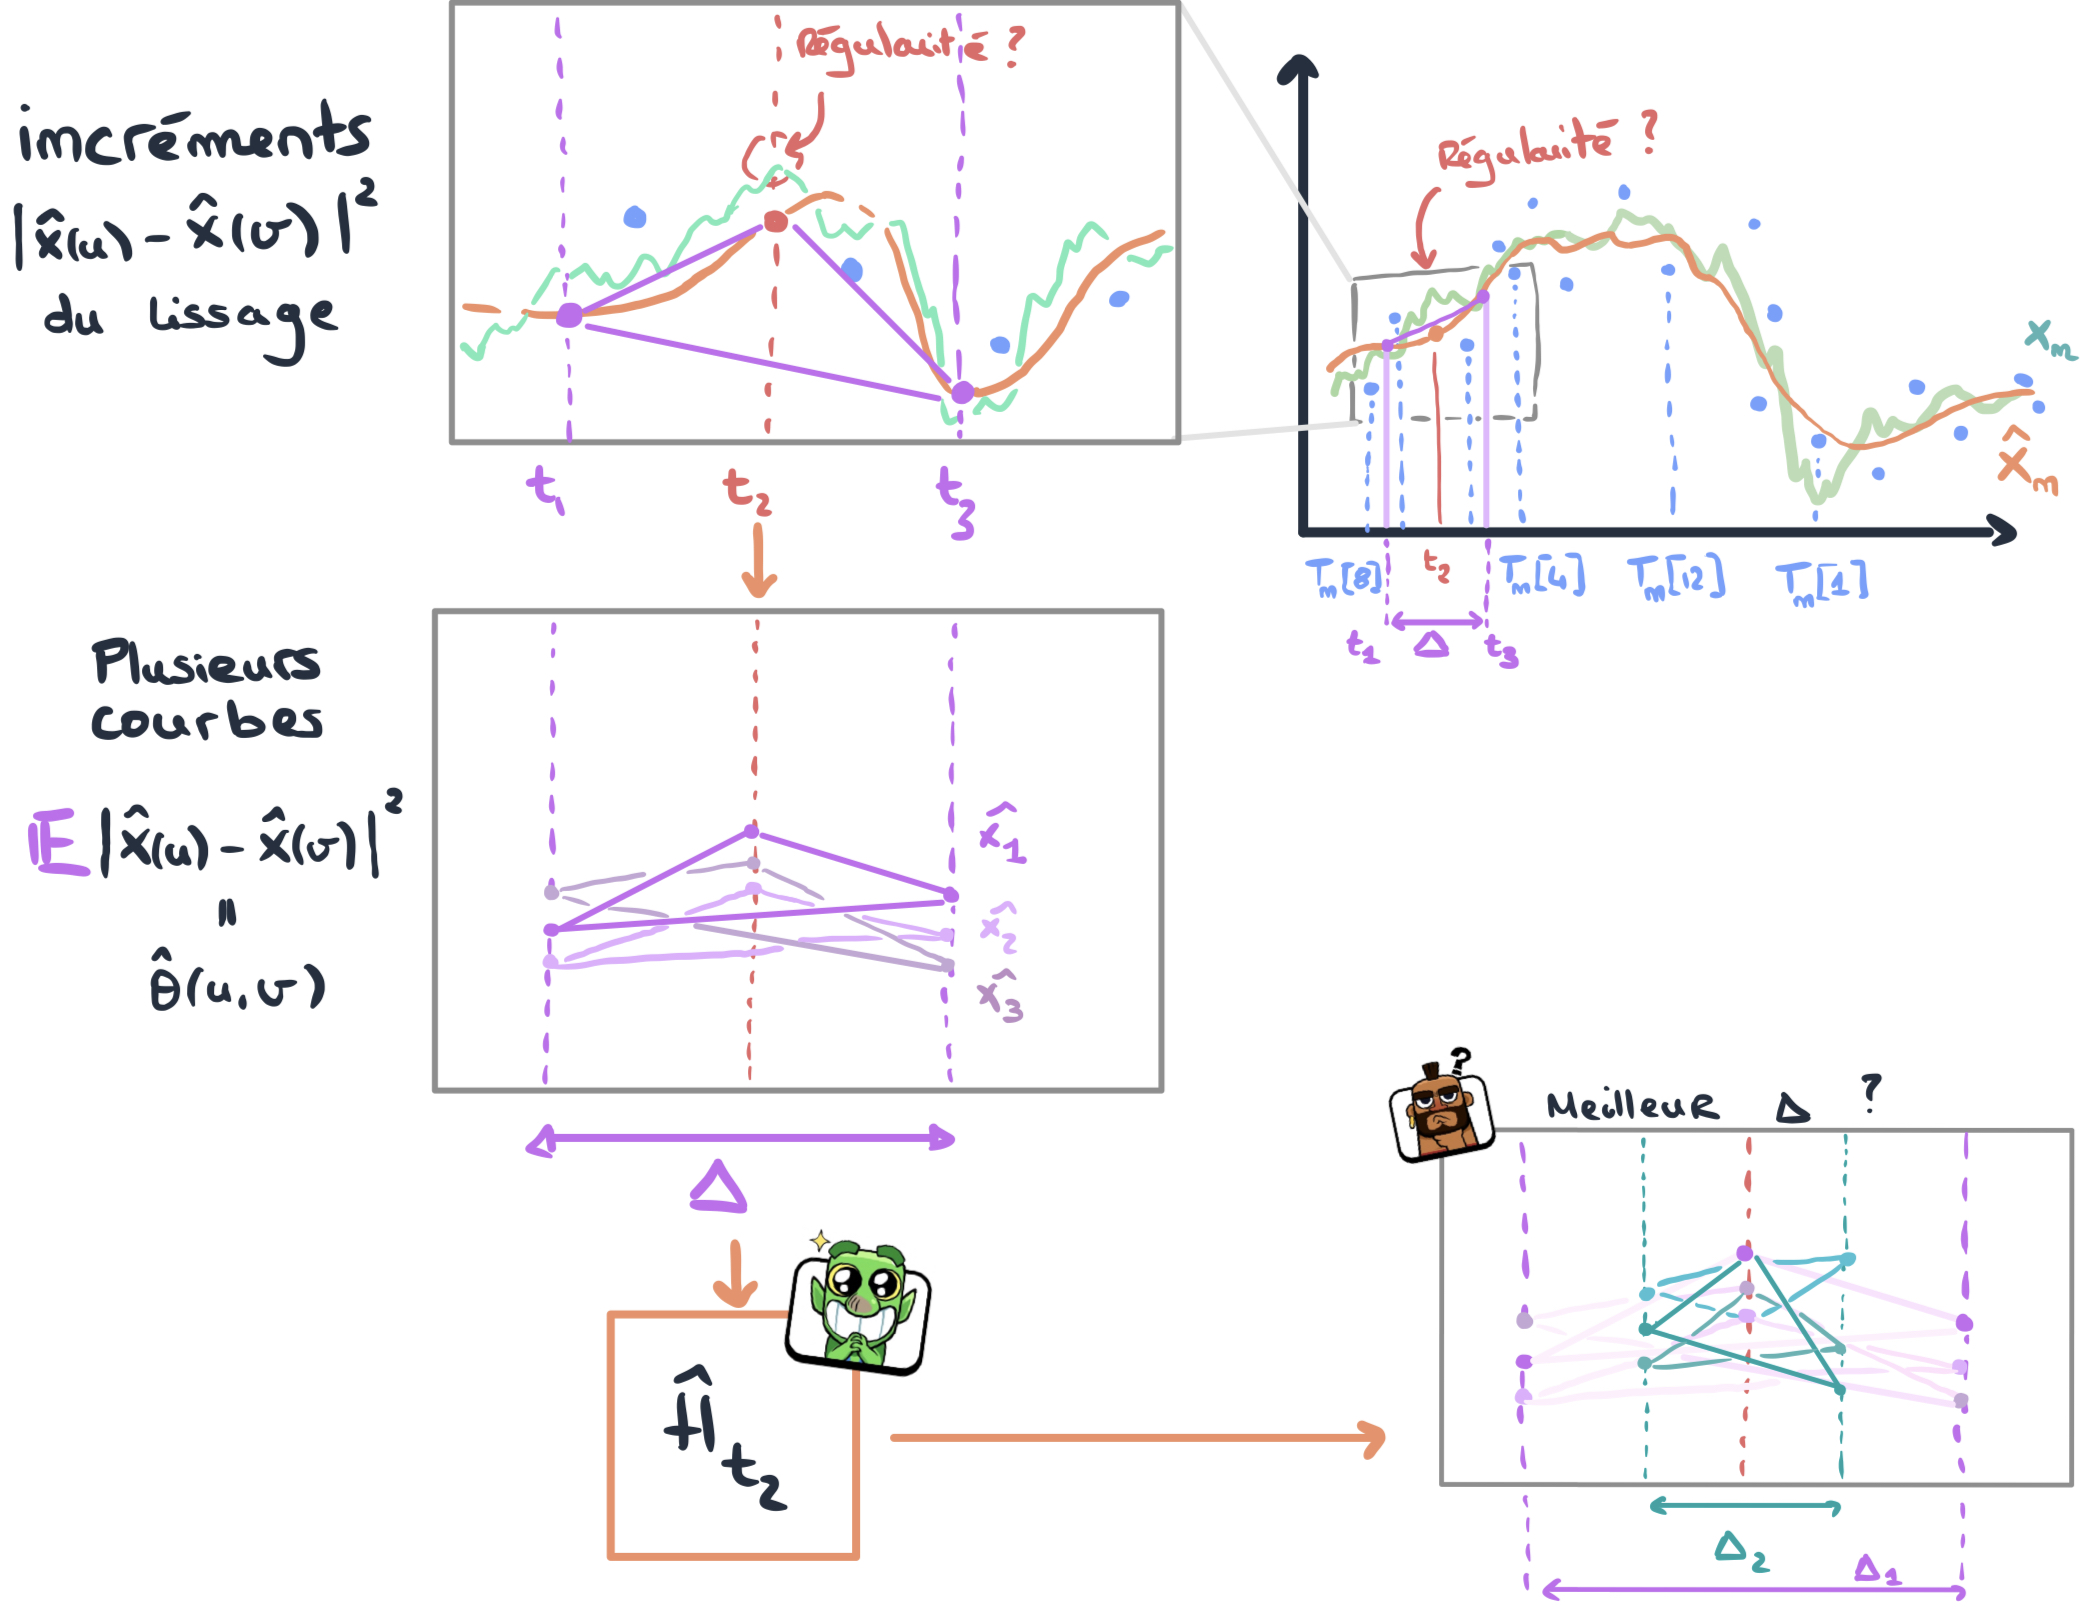
\includegraphics[width=\textwidth]{Images/sketches/estim_reg.jpg}
	\end{center}

	\caption{Schéma résumé de la méthode d'estimation de la régularité}
	\label{fig:sketch_estim_reg_methodo}
\end{figure}

La procédure d'obtention de la régularité est ainsi la suivante :

$\circled 1$ : Pré-lissage de la courbe

$\circled 2$ : Calcul des incréments quadratiques sur la courbe lissée

$\circled 3$ : moyennage des incréments (converge vers l'espérance sous hypothèse de dépendance faible)

$\circled 4$ : Utilisation de l'estimateur

Ce que nous cherchons désormais à déterminer est désormais la réponse à la question suivante :

\question{
	Quel $\Delta$ choisir pour obtenir la meilleure estimation de $H$ en $t_2$ ?
}

Pour étudier cela, nous allons simuler des données FAR(1) Höldériennes de régularité connue et allons étudier quel $\Delta$ fournit la meilleure estimation des paramètres de régularité en fonction de $\lambda$, $N$, $H_t$, ... \footnote{on pourra se référer à \ref{tab:model} pour la signification des notations}



\section{Simulation}
\label{sec:simulation}
\subsection{Objectifs de la simulation}
\label{subsec:sim-objectif}
L'objectif de la simulation est de pouvoir analyser le comportement des estimateurs des paramètres de régularité lorsque l'on fait varier $\Delta$, le diamètre du voisinage $J_\Delta$ dans lequel on vient utiliser de l'information pour capter la régularité. Cela permettra ensuite d'analyser cette fois le comportement de $\Delta^*$, le $\Delta$ optimal pour l'estimation des paramètres de régularité.

Jusqu'alors, on s'est surtout préoccupé d'expliquer l'intérêt et la méthodologie associée à l'obtention de la régularité. Toutefois différentes questions se posent vis-à-vis de cette estimation, notamment en lien avec le choix du $\Delta$ :

\question{
	$\circled 1$ : Le risque associé à l'estimation des paramètres de régularité, est il une fonction convexe (voire strictement convexe) de $\Delta$ ? Sinon, l'est-elle au moins au voisinage du $\Delta^*$ optimal pour l'estimation de la régularité ?

	\bigskip

	$\circled 2$ : Quel lien, si il en existe un, y-a-t-il entre $\Delta^*$ et d'autres quantités susceptibles d'affecter la vitesse de convergence de l'estimateur : $N$, $\lambda = \esperance{M_n}$, $H_{t_2}$, ... ?

	\bigskip

	$\circled 3$ : Peut-on fournir une procédure simple de détermination d'un $\Delta$ proche du $\Delta^*$ optimal, pouvant être obtenu à partir des données pour être utilisé en pratique par les statisticiens ?
}

\subsection{Mouvement Brownien Multi-Fractionaire (mfBm)}
\label{subsec:mfbm}
Afin de simuler un processus Höldérien non dérivable, on choisit de simuler un mouvement Brownien Multi-Fractionnaire. En effet il s'agit d'un processus qui, presque-sûrement, est continu mais différentiable nulle part. Le mouvement brownien multi-fractionnaire est d'autant plus intéressant dans le cadre de la simulation car on sait le générer en contrôlant localement sa régularité sur un voisinage $V$ de $t_0$.

\begin{equation*}
	\forall u,v \in V \quad	\esperance{ | \xi_n(u) - \xi_n(v) |^2 } \mathbf{\simeq} L_{H_{\xi}(t_0) } |u - v|^{2 H_{\xi}(t_0)}
\end{equation*}

Le lecteur pourra, si il le souhaite trouver plus de ressources, définitions et propriétés formelles sur le mouvement brownien fractionnaire et multi-fractionnaire en annexe \ref{annexe:brownien}. Le point essentiel exploité par l'algorithme utilisé pour la simulation est le suivant : le mouvement brownien multi-fractionnaire est un processus gaussien dont on sait expliciter la covariance en fonction de la régularité des instants considérés :

$$
	C(t,s) = D(H_{s},H_{t})\left[s^{H_{s}+H_{t}}+t^{H_{s}+H_{t}}-|t-s|^{H_{s}+H_{t}}\right]
$$

avec :
$$
	D\bigl(x,y\bigr) = \frac{{\sqrt{\Gamma(2x+1)\Gamma(2y+1)\sin(\pi x)\sin(\pi y)}}}{2\Gamma(x+y+1)\sin(\pi(x+y)/2)}
$$

il nous suffit donc de déterminer la matrice suivante :

$$
	\Sigma = \begin{bmatrix}
		\ddots &                                                                                                                  &
		\\
		       & D\bigl(H(t_i), H(t_j) \bigr)\cdot( t_i^{H(t_i) + H(t_j)} + t_j^{H(t_i) + H(t_j)} - |t_i-t_j|^{H(t_i) + H(t_j)} ) &
		\\
		       &                                                                                                                  & \ddots
	\end{bmatrix}
$$

avec :

\begin{equation*}
	t_i, t_j \in
	\mathds T = \left\{
	\underbrace{
		\begin{array}{c}
			t_1(\Delta, t), \, t_2(t), \, t_3(\Delta, t )
			\\
			t \in \vec t \quad \Delta \in \overrightarrow \Delta
		\end{array}
		%   \begin{array}{c}
		% 	 t_1^{[\,1\,]}(\Delta_1) \dots t_1^{[\,1\,]}(\Delta_p)
		% 	 \\
		% 	 \vdots
		% 	 \\
		% 	 {t_1^{[\,6\,]}(\Delta_1) \dots t_1^{[\,6\,]}(\Delta_p)}
		% 	 \\
		% 	\\
		% 	\overbrace{t_2^{[\,1\,]} \dots  \, t_2^{[\,6\,]}}^{\textsf{points où on évalue la régularité}}
		% 	\\
		% 	\\
		% 	t_3^{[\,1\,]}(\Delta_1) \dots t_3^{[\,1\,]}(\Delta_p)
		% 	\\
		% 	\vdots
		% 	\\
		% 	t_3^{[\,6\,]}(\Delta_1) \dots t_3^{[\,6\,]}(\Delta_p)
		%   \end{array}
	}_{
	\textsf{estimateur de régularité}
	}
	\quad , \,
	\underbrace{
		g_1 \dots g_G
	}_{
	\textsf{grille pour l'} \int \textsf{ de la relation FAR}
	}
	, \,
	\underbrace{
	T_n[\,1\,] \dots T_n[\,M_n\,]
	}_{
	\textsf{points observés (aléatoire)}
	}
	\right\}
\end{equation*}

Pour simuler un mouvement brownien multi-fractionnaire en les points désirés, il convient donc de simuler une loi normale multivariée d'espérance nulle et de covariance $\Sigma$.

\begin{rem}[complexité de la simulation]
	La méthode de génération du mouvement brownien multi-fractionnaire via une loi normale multi-variée implique l'inversion d'une matrice de covariance. La méthode utilisée pour l'inversion de cette matrice par la fonction \mintinline{R}{MASS::mvrnorm} utilisée pour la simulation est via la décomposition spectrale de celle-ci.

	\citer{
		The matrix decomposition is done via \mintinline{R}{eigen}; although a Choleski decomposition might be faster, the eigendecomposition is stabler.

		\begin{flushright}
			- Documentation du package R MASS~\cite{R-MASS}
		\end{flushright}
	}
	L'inversion de la matrice de covariance via sa décomposition spectrale est un algorithme de complexité $\grando{{(\operatorname{card}\mathds T)}^3}$. Ce qui implique qu'évaluer de plus en plus de point sur le même processus devient rapidement cher en calcul.
	\label{rem:inversion_matrice_covariance_mfbm_informel}
\end{rem}


\subsection{génération d'un $\operatorname{FAR}(1)$}
\label{subsec:far}

Parmi les avantages de l'utilisation d'un mouvement brownien multi-fractionnaire à simuler pour analyser le comportement du $\Delta$ se trouve le fait que l'on peut dériver facilement la régularité des courbes d'une relation $\operatorname{FAR}(1)$ basée sur ce processus. En effet, si l'opérateur linéaire de cette relation $\phi$ est un opérateur intégral $X \mapsto \int \beta(u,t) X(u)du$, il suffit alors que $H_\beta > H_\xi$ pour que le $\operatorname{FAR}(1)$ hérite de la régularité du mouvement brownien multi-fractionnaire. Ainsi on dispose directement de la régularité de notre $\operatorname{FAR}(1)$ en chaque point du support, ce qui s'avère très utile pour analyser les résultats.

Afin de générer la $N^{eme}$ observation d'un $\operatorname{FAR}$ définie par la relation auto-regressive suivante :

\begin{equation}
	X_N(t) = \int \beta(u,t)X_{N-1}(u)du + \varepsilon_N(t) \label{eq:rel_far_sim}
\end{equation}

Ainsi, il nous suffit de générer $N$ mouvements browniens multi-fractionnaires indépendants aux points dont on a besoin l'évaluation du mouvement brownien :

\begin{equation*}
	(\xi_1 , \xi_2, \dots , \xi_N ) \sim \operatorname{mfBm}(H, L)
\end{equation*}



\noindent que l'on utilise comme innovations dans la relation $\operatorname{FAR}(1)$ $\bigl[$eq. ~\ref{eq:rel_far_sim}$\bigr]$. La méthode de calul numérique de l'intégrale sélectionnée est la \emph{méthode des rectangles au point médian} car il s'agit de la méthode de calcul numérique d'intégrale de plus grand ordre avec $1$ unique point d'évaluation requis pour le calcul, ce qui est primordial vis à vis de la remarque formulée dans la section \ref{rem:inversion_matrice_covariance_mfbm_informel}.

\bigskip

Afin d'atteindre La stationnarité, on effectue une période de \og Burn-in \fg où l'on génère un nombre d'éléments (100) non retenus dans l'échantillon sauvegardé. en appelant $B$ le nombre d'étape de burn-in, on génère donc $N+B$ mouvements browniens $(\xi_1 , \dots ,\xi_B, \dots \xi_{N+B} )$ multi-fractionnaires indépendants aux points désirés, on applique à chaque itération la relation $\operatorname{FAR}(1)$ et on ne retient que les $N$ dernières itérations.

\bigskip

\noindent L'algorithme utilisé pour la génération du $\operatorname{FAR}(1)$ basée sur un opérateur intégral comme défini par la relation \ref{eq:rel_far_sim} est disponible en annexe : Algorithme \ref{alg:gen_far_grid}.


\section{Critère de sélection du Δ}
\label{sec:choix_risque_couple}

L'estimation des paramètres de régularité locale en $t_2$ ( $H_{t_2}$ et $L_{t_2}$ ) utilise les incréments quadratiques $\theta$ entre les différents points $t_1, t_2, t_3$ situés dans un voisinage de diamètre $\Delta$ autour de $t_2$.
En observant que $L$ est estimée par une expression impliquant $\theta$ et $\Delta^{2 H}$, d'une part, et le fait que $H$ est utilisé dans l'estimation adaptative d'une multitude de quantités qui intéressent le statisticien (covariance, ...) : une estimation précise de $H$ paraît plus cruciale pour la bonne estimation conjointe des deux quantités. 

\question{
	\smallskip\centering
	Doit-t-on se concentrer sur l'estimation de $H$ ou de $\theta$ ?
}

Les incréments quadratiques $\theta$ sont utilisées à la fois pour l'estimation de $H$ et de $L$. Nous allons donc chercher à déterminer un $\Delta$ adapté à l'estimation des incréments quadratiques. En effet, un mauvaise estimation des incréments induirait une mauvaise estimation de $H$. Puisque l'on a déterminé qu'une bonne estimation de $H$ était cruciale, et que cette quantité utilise deux valeurs d'incréments distinctes, nous allons nous focaliser sur l'estimation d'un couple de $\theta$ que nous noterons $\Theta$.

\bigskip

Le but étant d'obtenir un $\Delta$ utile en pratique, nous réalisons une simulation de Monte-Carlo avec $mc=200$ réplications indépendantes de la procédure d'estimation des paramètres de régularité locale. Et nous cherchons alors à déterminer quel $\Delta$ est meilleur en pratique sur les données simulées.

\bigskip

La métrique que nous allons sélectionner est \emph{la distance euclidienne entre une estimation d'un tel couple $\Theta$, que l'on nomme $\widehat \Theta$ et l'estimateur de l'espérance via la moyenne empirique des courbes non bruitées, observées pleinement, \textbf{relativement} à la cible de l'estimation $\widetilde \Theta$}. En effet, il s'agit du meilleur estimateur de l'espérance que l'on pourrait espérer atteindre (du biais est introduit lors du lissage non paramétrique des courbes bruitées). On considère donc le risque suivant :


\begin{equation}
	{\mathds E_p} \frac{{\distnorme 2 {\widehat \Theta\bigl[\, p \,\bigr]} {\widetilde \Theta \bigl[ \,p \,\bigr]}}^2}{{\norme 2 {\widetilde \Theta \bigl[ \,p \,\bigr]}}^2}
	=
	{\mathcal R}^{[\,rel\,]} \bigl( \, \Theta \, , \, \Delta \, \bigr)
	\simeq
\widehat{\mathcal R}^{[\,rel\,]} \bigl( \, \Theta \, , \, \Delta \, \bigr)
	=
	\frac 1 {mc} \sum\limits_{p=1}^{mc} \frac{{\distnorme 2 {\widehat \Theta\bigl[\, p \,\bigr]} {\widetilde \Theta \bigl[ \,p \,\bigr]}}^2}{{\norme 2 {\widetilde \Theta \bigl[ \,p \,\bigr]}}^2}
\end{equation}

\begin{figure}[H]
	\centering
	\begin{minipage}{0.65\textwidth}
		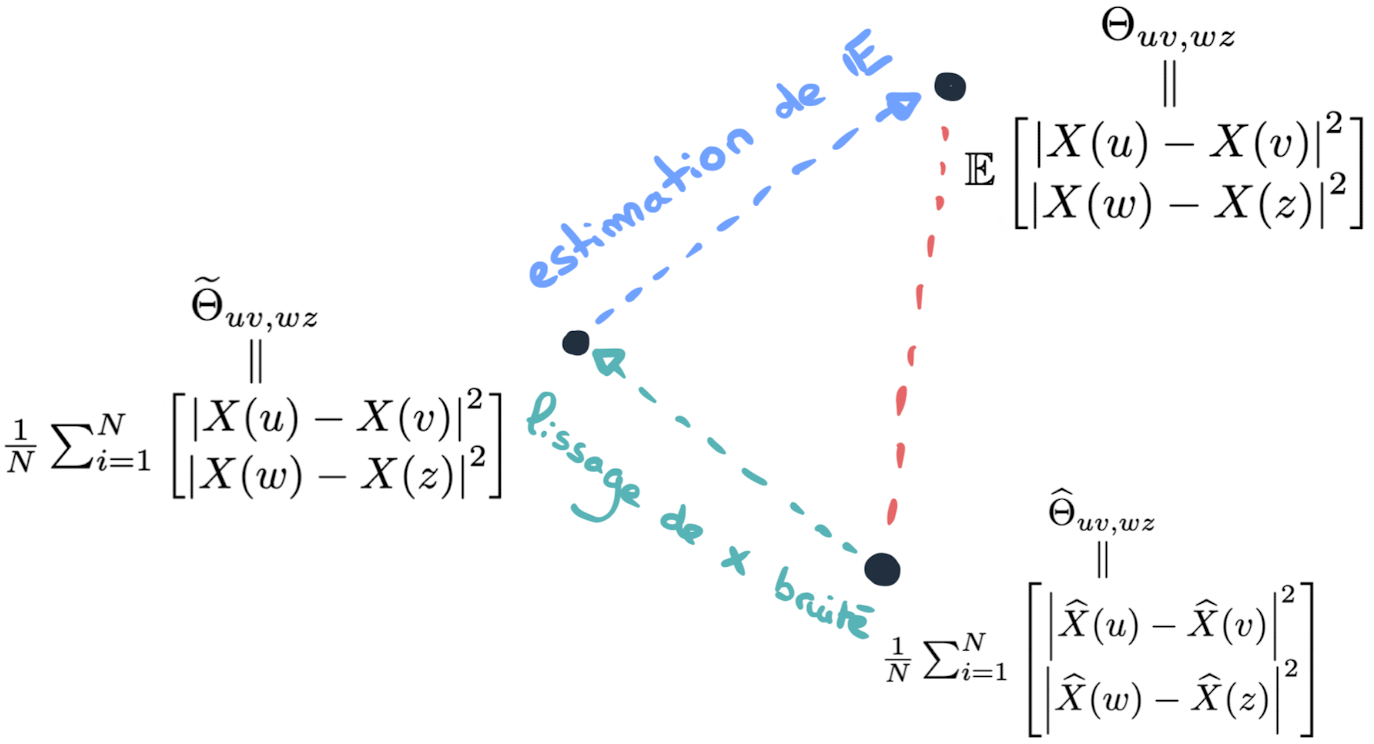
\includegraphics[width=0.8\textwidth]{Images/sketches/theta_biais.png}
	\end{minipage}
	\begin{minipage}{0.3\textwidth}
		Dans la formulation du risque, 
		$[p]$ désigne la $p^{eme}$ réplication de Monte-Carlo de la quantité considérée.
	\end{minipage}
	\caption{Schéma représentant les différentes approximations du couple d'incréments}
	\label{fig:sketch_theta_biais_corpus}
\end{figure}
